%************************************************
\chapter[Application du modèle à l'évaluation]{Application du modèle morphologique à l'évaluation des algorithmes d'analyse automatique de scènes sonores environnementales}\label{ch:ml_simuperf}
%************************************************

\section{Introduction}

\gl{TODO: un point méthodologique, ici corpus de scènes et non corpus d'objets, du coup chaque scène est un sous corpus, du coup on a une métrique par scène et une métrique moyenne par corpus, du coup théorème centrale limite, du coup test paramétrique, du coup on s'éloigne des recommandations de \citep{demvsar2006statistical}}

%%%%%%%%%%%%%%%%%%%%%%%%%%%%%%%%%%%%%%%%%%%%%%%%%%%%%%%%%%%%%%%%%%%%%%%%%%%%%%%%%%%%%%%%%%%%%%%
%%%%%%%%%%%%%%%%%%%%%%%%%%%%%%%%%%%%   DCASE 2013   %%%%%%%%%%%%%%%%%%%%%%%%%%%%%%%%%%%%%%%%%%%
%%%%%%%%%%%%%%%%%%%%%%%%%%%%%%%%%%%%%%%%%%%%%%%%%%%%%%%%%%%%%%%%%%%%%%%%%%%%%%%%%%%%%%%%%%%%%%%

\section{Application au challenge DCASE  2013}

\subsection{Objectif}

\gl{L'objectif dans cette étude est de ré-évaluer les algorithmes soumis dans le cadre de la tâche 2 de détection d'événements sonores (AED) du challenge DCASE 2013\footnote{Par souci de lisibilité, nous nous préciserons plus par la suite la tâche du challenge DCASE à laquelle nous faisons référence. Le lecteur comprendra que pour la totalité de ce chapitre, l'appellation ``\,challenge DCASE\,'' désigne la tâche 2 de détection d'événements (AED) dudit challenge.} (\cf~Section~\ref{sec:ch6_challengeDcasePresentation}).}

\gl{Plus précisément, nous voulons tester la capacité de généralisation de ces algorithmes, \ie~leur aptitude à maintenir des performances de détection similaires sur plusieurs corpus de scènes présentant des conditions expérimentales différentes.}

La capacité de généralisation est considérée suivant deux angles:

\begin{itemize}
\item robustesse à la diversité structurelle: évaluer la capacité de généralisation sur des corpus de scènes composés des mêmes samples, mais dont les caractéristiques structurelles (intensité sonore des samples, positionnement/espacement moyen des samples) diffèrent;
\item robustesse à  la diversité des samples: évaluer la capacité de généralisation sur des corpus de scènes possédant les mêmes caractéristiques structurelles (intensité sonore des samples, positionnement des samples), mais composés d'une sélection de samples différents. Par ``\,sample différent\,'', nous entendons des enregistrements d'événements sonores différents, mais appartenant à la même classe (\eg~claquement de porte).  En effet, quand on considère une tâche de classification, un problème de taille est de savoir si le système évalué est capable de généraliser ses capacités de classification à des données non-observées, mais qui correspondent aux classes considérées dans les corpus d’entraînements et de développement.
\end{itemize}

La méthode suivie consiste à utiliser le modèle de scènes sonores proposé (\cf~Section~\ref{sec:ch4_modelForm}) afin de générer de nouveaux corpus de scènes simulées, scènes dont nous contrôlons les structures internes, ainsi que la nature des samples utilisés. 

\gl{Afin d'évaluer la robustesse des algorithmes à la présence de nouveaux samples, nous considérons les performances obtenues sur des corpus de scènes, simulées avec une  banque de données de sons isolés dont les samples (événements et \emph{background}) ont été enregistrés dans des environnements acoustiques différents de ceux du corpus d'évaluation d'origine du challenge DCASE 2013. L'enregistrement de cette nouvelle banque de données a été effectué dans le cadre de cette étude.}

Il s'agit alors d'éprouver les algorithmes sur ces nouveaux corpus, et de comparer leurs performances avec celles obtenues sur le corpus d'origine. Les différences nous permettent de conclure quant à la capacité de généralisation des algorithmes considérés.

\subsection{Génération des corpus}

\begin{table}[t]
\begin{center}
\begin{tabular}{lcc}
\textbf{Index} & \textbf{Nom}  & \textbf{Description}  \\ 
\hline
1   & porte-frapper & Frapper à la porte \\
2   & porte-claquer & Claquer la porte \\
3   & parole        & Personne prononçant \\
    &               &  une phrase \\
4   & rire          & Personne riant  \\    
5   & gorge         & Personne se   \\
    &               & raclant la gorge \\
6   & toux          & Personne toussant \\
7   & tiroir        & Ouverture/fermeture d'un tiroir \\
8   & imprimante    & Bruit d'une imprimante \\
9   & clavier       & Bruit des touches d'un clavier \\
10  & souris        & Bruit d'un clic de souris \\
11  & stylo         & Poser un stylo sur une table \\
12  & bouton        & Bouton permettant d'allumer la lumière \\
13  & clefs         & Poser un jeu de clefs sur une table \\    
14  & téléphone     & Sonnerie de téléphone \\
15  & alerte        & bruit d'une alerte \\
    &               & électronique (ordinateur, mobile) \\
16  & page          & Tourner une page \\     
\hline      
\end{tabular}
\end{center}
\caption{Classes d'événements sonores utilisées dans le cadre du challenge DCASE 2013}
\label{tab:eventDCASE2013}
\end{table}

Cette section décrit les différents corpus de scènes simulées utilisés lors de l'expérience. 

Tous les corpus de scènes simulées sont générés à partir des scènes enregistrées du corpus \emph{test-QMUL} : le corpus de \emph{test} de la tâche de détection d'événements (AED) du challenge DCASE 2013  \citep{giannoulis2013detection} (\cf~Section~\ref{sec:ch6_dcase2013AED}). 

\emph{test-QMUL} a été enregistré à l'université \emph{Queen Mary University of London}. Il est composé de 11 enregistrements d'ambiances de bureau, tous d'une durée proche de la minute. Chaque scène est une séquence d'événements sonores non enchevêtrés. Ces événements sont repartis en 16 classes de sons, classes détaillées dans le tableau~\ref{tab:eventDCASE2013}. Les enregistrements ont été effectués dans 5 environnements acoustiques différents. Les scènes sont annotées par deux individus différents. Pour chaque scène, et à chaque événement entendu, l'annotateur indique la classe de l'événement, son \emph{onset} (la position du début de l'événement) et son \emph{offset} (la position de fin de l'événement). Toutes les annotations sont utilisées. Les 22 couples scène-annotateur permettent de composer une vérité terrain.

À partir des annotations de \emph{test-QMUL}, quatre corpus de scènes simulées sont générés, mettant en œuvre deux banques de données de sons isolés, ainsi que deux processus de simulation distincts. Les banques de données de sons isolés, ainsi que les processus de simulation sont détaillés dans les sections suivantes (\cf~Sections~\ref{sec:ch7_eventDataset},~\ref{sec:ch7_simuProcessInstance} et~\ref{sec:ch7_simuProcessAbstract}). 

\begin{figure}[t]
\begin{center}
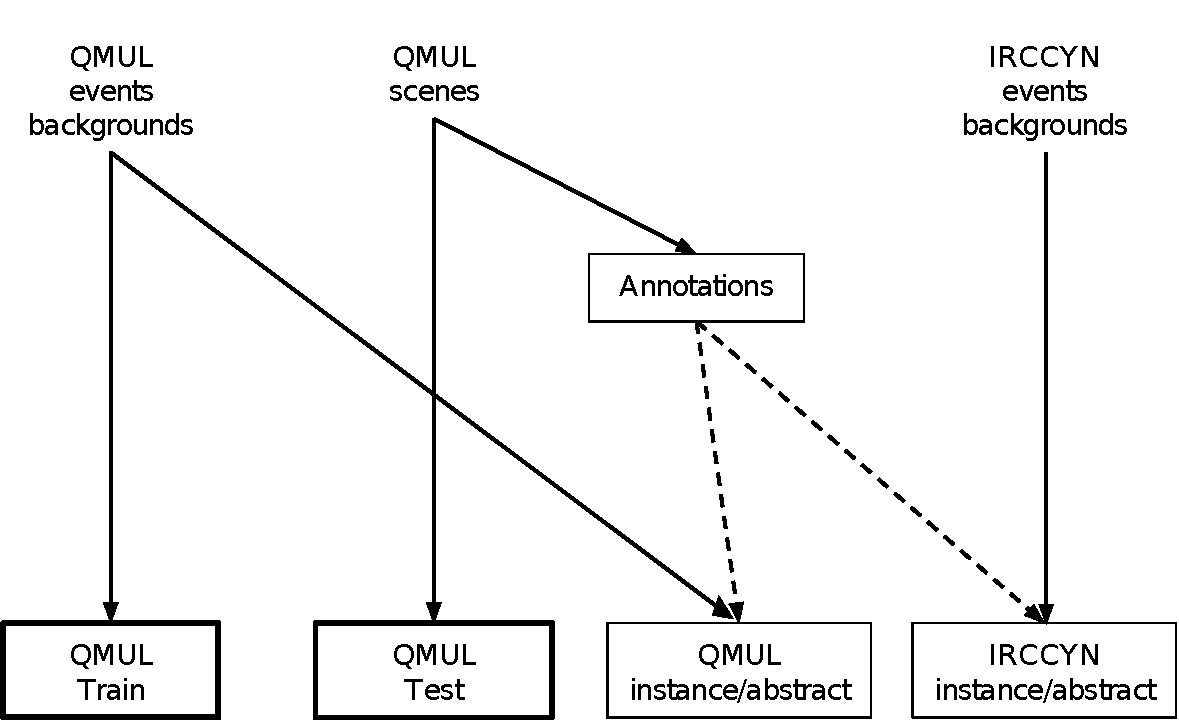
\includegraphics[width=1\textwidth]{gfx/ch_7/databasesTasslp.pdf}
\label{fig:databasesDCASE2013Simu}
\caption{Generation process of the corpora considered in this evaluation. As part of the DCASE challenge, systems were trained on QMUL Train and tested on QMUL Test during the DCASE challenge.} 
\end{center}
\end{figure}

\subsubsection{Banque de données de sons isolés \emph{QMUL} et \emph{IRCCYN}}
\label{sec:ch7_eventDataset}

Deux banques de sons isolés sont utilisées pour générer les scènes isolées. Elles sont respectivement nommées \emph{QMUL} et \emph{IRCCYN}. Toutes deux sont composées de deux types de sons:

\begin{itemize}
\item les événements: les enregistrements de sons isolés devant être détectés et identifiés par les algorithmes;
\item les \emph{backgrounds}: les enregistrements de fonds sonores, \ie~des scènes amorphes (textures ne possédant pas d'événement saillant, \cf~Section~\ref{sec:ch4_eventTextureAmorphe}) rendant compte de l’environnement acoustique naturel du lieu d'occurrence des événements. 
\end{itemize}

Les sons isolés de la banque \emph{QMUL} sont extraits de scènes enregistrées à l'université \emph{Queen Mary University of London} (QMUL) dans le cadre de la préparation du challenge AED DCASE-2013, mais n'ayant pas été utilisées lors de l'évaluation, \ie~ne faisant pas partie des corpus d'évaluation (\emph{test-QMUL}) et de développement. Ces sons isolés profitent donc des mêmes conditions d’enregistrement que les scènes du corpus \emph{test-QMUL} \citep{Giannoulis2013database}. Le nombre d'événements par classe varie de 3 à 23. Les enregistrements de \emph{backgrounds} ont été réalisés sur les mêmes environnements acoustiques que ceux utilisés pour le corpus \emph{test-QMUL}, avec là encore les mêmes conditions d'enregistrements.

La banque \emph{IRCCYN} est une nouvelle banque de sons isolés, enregistrés à l'Institut de Recherche en Cybernétique de Nantes (IRCCyN). Cette dernière comprend les mêmes classes que celles présentes dans le corpus \emph{test-QMUL} (\cf~Tableau~\ref{tab:eventDCASE2013}). Les enregistrements ont été effectués dans un environnement calme, à l'aide d'un micro canon \emph{AT8035} connecté à un enregistreur \emph{ZOOM H4n}. Chaque classe est composée de 20 événements sonores, ce qui correspond au nombre d'événements disponibles dans le corpus d'entraînement du challenge DCASE-2013 \citep{Giannoulis2013database,giannoulis2013detection}. Les \emph{background} ont été enregistrés de nuit, dans les bureaux de l'IRCCyN, afin qu'ils ne soient pas pollués par des bruits non souhaités. \\

\gl{TODO: détailler la banque de données IRCCYN}

\subsubsection{Processus de simulation instance}
\label{sec:ch7_simuProcessInstance}

Pour le processus de simulation \emph{instance}, l'objectif est de générer des scènes simulées qui ressemblent le plus possible aux scènes du corpus \emph{test-QMUL}. Cette ressemblance s'entend sous deux aspects:

\begin{itemize}
\item \emph{la structure temporelle}: le positionnement temporel en terme d'\emph{onsets} des événements sonores;
\item \emph{les niveaux sonores des événements}: la puissance du ratio entre l'énergie de l'événement et celle du \emph{background}, notée EBR (\emph{event to Background power Ratios}). L'$EBR$ d'un événement de $N$ échantillons est obtenu en calculant le ratio en décibels entre de la valeur efficace (niveau $RMS$, \cf~Section~\ref{sec:ch5_recordDataSet}) du signal (\cf~Équation~\ref{eq:ch7_eq2}) de l'événement ($E_{rms}$) et du \emph{background}  $B_{rms}$):

\begin{equation}
\label{eq:ch7_eq1}
EBR=20log_{10} \left(  \dfrac{E_{rms}}{B_{rms}} \right) 
\end{equation}

\begin{equation}
\label{eq:ch7_eq2}
X_{rms}=\sqrt{\dfrac{1}{N} \sum_{n=1}^{N} x(n)^2}
\end{equation}

$x(n)$ peut être remplacé par $e(n)$ ou $b(n)$, respectivement les valeurs des signaux de l'événement et du \emph{background} en volt à l'échantillon $n$. 
\end{itemize}

Pour chaque événement, et chaque couple scène-annotateur du corpus \emph{test-QMUL}, nous extrayons les positions d'\emph{onsets} et d'{offsets}, et calculons une approximation de l'$EBR$. Comme il n'est pas possible d'isoler le signal du \emph{background} des scènes de \emph{test-QMUL}, $B_{rms}$ est obtenu à partir des périodes dénuées d'événements. \\
 
\gl{TODO: expliquer comment on supprime le niveau de bruit dans $E_{rms}$} \\

Les positions \emph{onsets} et les $EBRs$ ainsi recouvrés sont utilisés pour simuler un nouveau corpus de scènes. Pour chaque scène simulée, à chaque \emph{onset} d'une annotation (couple scène-annotateur), nous plaçons un événement de la même classe, choisi aléatoirement parmi la banque de sons isolés (\emph{QMUL} ou \emph{IRCCYN}). Afin de garantir que les samples ne soient pas trop longs, ces derniers sont coupés s'ils dépassent d'au moins $0.5$ la durée de l'annotation. Les niveaux des événements des scènes simulées sont fixés par rapport aux $EBRs$ calculés sur les scènes enregistrées. 

Le processus de simulation \emph{instance} ne s'appuie donc pas sur le modèle introduit à la section~\ref{sec:ch4_modelForm}. L'objectif ici est d’obtenir des scènes simulées possédant des samples différents des scènes enregistrées, mais dont les structures temporelles et les $EBRs$ sont aussi proches que possible de ceux des scènes du corpus \emph{test-QMUL}.

\subsubsection{Processus de simulation abstract}
\label{sec:ch7_simuProcessAbstract}

L'objectif du processus de simulation \emph{abstract} est de capturer les paramètres haut niveaux régissant la structure de la scène enregistrée, et de les utiliser afin de régénérer cette dernière. Le processus \emph{abstract} s'appuie sur le modèle introduit à la section~\ref{sec:ch4_modelForm}. Concrètement, le modèle est instancié suivant des paramètres $\mu_i^a$, $\sigma_i^a$, $\mu_i^t$ et $\sigma_i^t$ (\cf~Équation.~\ref{eq:ch4_eq1} et~\ref{eq:ch4_eq2}) estimés sur la scène enregistrée. Pour chaque couple scène-annotateur du corpus  \emph{test-QMUL}, ces paramètres sont estimés à partir de l'annotation ($\mu_i^t$ et $\sigma_i^t$) et du signal ($\mu_i^a$ et $\sigma_i^a$). Les $EBRs$ et les espacements inter-\emph{onsets} de la scène simulée sont alors obtenus à partir des distributions normales $\mathcal{N}(\mu_i^a,\sigma_i^a)$ et $\mathcal{N}(\mu_i^t,\sigma_i^t)$ respectivement. Pour chaque classe, le début et la fin des pistes des scènes simulées sont les mêmes que ceux des scènes enregistrées.

Comme pour le processus de simulation \emph{instance}, les événements sont choisis aléatoirement. Afin de garantir que les durées des événements des scènes simulées ne soient pas trop long par rapport à ceux des scènes enregistrées, la durée $D$ d'un sample d'une classe $i$ est seuillé si:

\begin{equation}
D-\mu_i^d-\sigma_i^d>5
\end{equation}

avec, $\mu_i^d$ et $\sigma_i^d$ les moyennes et écarts types des durées des samples appartenant à la classe $i$ pour une annotation donnée. La limite de 5 secondes permet de minimiser l'impact d'une telle opération de seuillage sur les sons impulsifs.

\subsubsection{Banque de données de scènes simulées}
\label{sec:ch7_datasetEtEbr}

Cinq corpus sont considérés pour l'évaluation (\cf~Figure~ref{fig:databasesDCASE2013Simu}), à savoir, le corpus de scènes enregistrées \emph{test-QMUL}, et quatre corpus de scènes simulées:

\begin{itemize}
\item \emph{instance-QMUL} (insQ);
\item \emph{abstrait-QMUL} (absQ);
\item \emph{instance-IRCCYN} (insI);
\item \emph{abstrait-IRCCYN} (absI).
\end{itemize}

Les labels ``\,QMUL\,'' et ``\,IRCCYN\,'' font référence aux banques de données de sons isolés utilisées pour générer les scènes simulées. Les labels ``\,instance\,'' et ``\,abstract\,'' désignent, eux, les processus de simulation utilisés. 

Afin d'évaluer l'influence du niveau relatif des événements par rapport au \emph{background} sur les performances des algorithmes, le corpus \emph{instance-QMUL} est composé de quatre sous-corpus appelés respectivement \emph{insQ-EBR(6)}, \emph{insQ-EBR(0)}, \emph{insQ-EBR(-6)} et \emph{insQ-EBR(-12)}. Pour \emph{insQ-EBR(0)}, les $EBRs$ estimés sur \emph{test-QMUL} sont préservés.  Pour \emph{insQ-EBR(6)}, \emph{insQ-EBR(-6)} et \emph{insQ-EBR(-12)}, des compensations de +6$dB$, -6$dB$, -12$dB$ sont ajoutées, lors de la simulation, aux $EBRs$ d'origines. A noter que pour ces sous-corpus, seul l'$EBR$ est modifié, les positions temporelles des événements, ainsi que les samples sélectionnés, sont strictement identiques entre les quatre sous-corpus.

Pour tous les corpus (\emph{abstract-QMUL}, \emph{instance-IRCCYN} et \emph{abstract-IRCCYN}), ainsi que les sous-corpus de \emph{instance-QMUL}, une simulation est réalisée pour chaque couple scène-annotateur de \emph{test-QMUL} ($11\times2=22$ couples). 

De plus, chaque simulation est répliquée 10 fois. A chaque réplication, la sélection aléatoire des samples varie. Pour les corpus générés suivant le processus de simulation \emph{abstract} (\emph{abstract-QMUL} et \emph{abstract-IRCCYN}), les $EBRs$ et espacements inter-\emph{onsets} des samples obtenus à partir des distributions normales  $\mathcal{N}(\mu_i^a,\sigma_i^a)$ et $\mathcal{N}(\mu_i^t,\sigma_i^t)$ sont également re-tirés d'une réplication à une autre \gl{TODO: A vérifier}. Chaque corpus/sous-corpus est ainsi composé de 220 scènes simulées ($11\times2\times10$).

Tous les corpus sont disponibles en ligne\footnote{Dataset URLs: \begin{itemize}
\item \emph{test-QMUL}: \url{https://archive.org/details/dcase2013_event_detection_testset_OL};
\item \emph{instance-QMUL}, \emph{abstract-QMUL}: \url{https://archive.org/details/dcase_replicate_qmul};
\item \emph{instance-IRCCYN}, \emph{abstract-IRCCYN}: \url{https://archive.org/details/dcase_replicate.
irccyn}
\end{itemize}} et ont été simulés à l'aide de l'outil de simulation MATLAB développé dans le cadre de cette thèse (\cf~Section~\ref{sec:ch4_modAnaAuto}).

\subsubsection{Analyse du réalisme des scènes simulées}

Afin d'évaluer le réalisme des scènes acoustiques simulées, une expérience sensorielle d'analyse sémantique différentielle est conduite. \\

\textbf{Procédure} \\

22 stimuli doivent être notés, comprenant 11 scènes enregistrées de \emph{test-QMUL} et 11 scènes simulées de \emph{instance-IRCCYN}. Les sujets doivent évaluer le réalisme de chaque scène suivant une échelle graduée de 7 points, allant de 1 (non réaliste) à 7 (très réaliste). 

L'ordre de présentation est différent pour chaque sujet. Les sujets doivent écouter la totalité d'une scène avant de se prononcer.

À la fin de l'expérience, les sujets sont invités à commenter librement leurs notations. \\

\textbf{Apparatus} \\

L'audio est diffusé en monophonique. Au début de l'expérience, il est demandé aux sujets d'utiliser un casque audio, et de régler le volume sonore à un niveau confortable.  \\

\textbf{Participant} \\

15 sujets ont participé à l'étude. Tous ont réalisé l'expérience avec succès. \\

\textbf{Résultats} \\

Nous considérons $\mathcal{R}_{sujet}$ les notes de réalisme par sujet, notes moyennées en considérant séparément les scènes de \emph{test-QMUL} et celles de \emph{instance-IRCCYN}.

Les $\mathcal{R}_{sujet}$ des scènes enregistrées et simulées sont respectivement de $4.4$ et $3.3$ (\cf~Figure~\ref{fig:xpRealism}). Les deux population présentent une différence significative (t-test appariées: $p<0.01$). D'après les commentaires des sujets, il semble que les scènes enregistrées n'aient pas été perçues comme très réalistes à cause de leur caractère scripté, les sujets ayant reconnu le fait qu'il s'agit de scènes jouées. 

En ce qui concerne les scènes simulées, les sujets ont rapporté que: 

\begin{itemize}
\item ``\,le fond sonore semble synthétique/artificiel\,'', bien que ce dernier ait été enregistré;
\item ``\,certains événements sont coupés\,''. Ce dernier point est en effet avéré. La coupe de certains événements est due à un choix de conception du corpus \emph{instance-IRCCYN} discuté à la section~\ref{sec:ch7_simuProcessInstance}. Ce choix est pris dans le but de minimiser la différence entre la scène simulée, et celle de référence. 
\end{itemize}

Il convient de noter que, pour de nombreux participants, certaines scènes simulées ont reçu une note de réalisme plus élevée que certaines des scènes naturelles, ce qui montre que, bien que des différences notables peuvent être faites, elles n'influencent le réalisme acoustique que dans une moindre mesure.

\begin{figure}[t]
\begin{center}
\includegraphics[width=.33\textwidth]{gfx/ch_7/xp_realism_2}
\caption{Distribution des notes de réalisme $\mathcal{R}_{sujet}$ pour les scènes enregistrés \emph{test-QMUL} et les scènes simulées \emph{instance-IRCCYN}}
\label{fig:xpRealism} 
\end{center}
\end{figure}

\subsection{Métrique}

La métrique considérée dans cette analyse est $Fcw_{eb}$ (\cf~Section~\ref{sec:ch6_metriqueAED}), \ie~la moyenne des F-mesures calculées séparément pour chaque classe, en tenant compte des \emph{onsets} des événements, et avec une fenêtre de tolérance de 100ms. Cette dernière a l'avantage: 

\begin{itemize}
\item d'être facilement interprétable;
\item de ne favoriser aucune classe.
\end{itemize}

\subsection{Données et analyses}

\gl{Pour le calcule des métriques, nous suivons la méthodologie suivie par le challenge DCASE 2013:}

\begin{itemize}

\item \emph{test-QMUL}: pour chaque scène, les performances mesurées sont moyennées suivant les deux annotateurs;
\item  \emph{instance-QMUL}, \emph{abstract-QMUL},  \emph{instance-QMUL} et \emph{abstract-QMUL}: pour chaque scène, les performances sont moyennées:

\begin{enumerate}
\item suivant les réplications (10 réplications par scène);
\item suivant les deux annotateurs.
\end{enumerate}

\end{itemize}

\gl{Cette approche nous laisse avec 11 observations (\ie~11 mesures de performances) par condition expérimentale (corpus et systèmes)}\footnote{À noter que la méthode adoptée dans ce document pour intégrer les performances des algorithmes diffère de celle utilisée dans la publication correspondante \citep{lafay2016morphological}. Les différences observées sont cependant minimes, et ne changent en rien les résultats et les conclusions.}.

L'analyse s'effectue en deux temps, suivant le corpus de sons isolés considéré:

\begin{itemize}

\item \gl{Corpus de sons isolés \emph{QMUL}: cette analyse considère les trois corpus \emph{test-QMUL}, \emph{instance-QMUL} et \emph{abstract-QMUL}. Elle a deux objectifs:}

\begin{enumerate}
\item \gl{évaluer si il existe des différences significatives entre les performances des algorithmes observées sur les corpus \emph{test-QMUL}, \emph{insQ-EBR(0)} et \emph{abstract-QMUL}. L'objectif ici est de vérifier que les algorithmes sont capables de généraliser les performances obtenues sur \emph{test-QMUL} pour des corpus simulés avec des sons isolées enregistrés dans les mêmes conditions que ceux de \emph{test-QMUL}, et dont les scènes possèdent une structure ($EBR$ et positions des \emph{onsets}) identique (\emph{insQ-EBR(0)}) ou similaire (\emph{abstract-QMUL}) à celles de \emph{test-QMUL}. Pour apprécier la significativité des différences observées, nous considérons une ANOVA à mesures répétées comportant 1 facteur intra-sujet (les systèmes) et 1 facteur inter-sujet (les corpus). L'analyse \emph{post hoc} s'effectue suivant une procédure de Tukey-Kramer;}

\item \gl{évaluer si il existe des différences significatives entre les performances des algorithmes observées sur les corpus \emph{insQ-EBR(6)}, \emph{insQ-EBR(0)}, \emph{insQ-EBR(-6)} et \emph{insQ-EBR(-12)}. L'objectif ici est de vérifier que les algorithmes sont capables de généraliser les performances obtenues sur \emph{insQ-EBR(0)} pour des corpus simulés identiques mais possédant des niveaux de bruits différents. Pour apprécier la significativité des différences observées, nous considérons une ANOVA à mesures répétées comportant 2 facteurs intra-sujet (les systèmes et les $EBR$). L'analyse \emph{post hoc} s'effectue suivant une procédure de Tukey-Kramer;}

\end{enumerate}

\item \gl{corpus de sons isolés \emph{IRCCYN}: cette analyse considère les trois corpus \emph{test-QMUL}, \emph{instance-IRCCYN} et \emph{abstract-IRCCYN}. L'objectif ici est de vérifier que les algorithmes sont capables de généraliser les performances obtenues sur \emph{test-QMUL} pour des corpus simulés avec des sons isolées enregistrés dans des conditions différentes de ceux de \emph{test-QMUL}, et dont les scènes possèdent une structure ($EBR$ et positions des \emph{onsets}) identique (\emph{instance-IRCCYN}) ou similaire (\emph{abstract-IRCCYN}) à celles de \emph{test-QMUL}.  Pour apprécier la significativité des différences observées, nous considérons une ANOVA à mesures répétées comportant 1 facteur intra-sujet (les systèmes) et 1 facteur inter-sujet (les corpus). L'analyse \emph{post hoc} s'effectue suivant une procédure de Tukey-Kramer.}

\end{itemize}

Pour les ANOVA à mesures répétées, la sphéricité est évaluée à l'aide d'un test de Mauchly. Si l'hypothèse de sphéricité est violée, la valeur $p$ est calculée à l'aide d'une correction de Greenhouse-Geisser (\cf~Annexe~\ref{app:anova}). Dans ce cas, nous notons $p_{gg}$ la valeur $p$ ainsi corrigée. L'analyse \emph{post hoc} est conduite en suivant la procédure de Tukey-Kramer, celle de Bonferroni étant jugée trop sévère pour le cadre de notre étude. Le seuil de significativité est fixé à $\alpha=0.05$ pour toutes les analyses.

\subsection{Système de détection}

\begin{figure}
\center
\tikzset{mynode/.style={rectangle,rounded corners,draw=black, top color=white, text centered},} 
\tikz \draw [o->] (0,0) -- (1\textwidth,0)
node[mynode, pos=0.15] {\footnotesize Pre-traitement$*$} 
node[mynode, pos=0.38]  {\footnotesize Descripteurs}
node[mynode, pos=0.6]  {\footnotesize Classifieurs} 
node[mynode, pos=0.85] {\footnotesize Post-traitement$*$} 
node[pos=0.15, below=10pt] {\footnotesize dé-bruitage} 
node[pos=0.38, below=10pt] {\footnotesize MFCCs} 
node[pos=0.6, below=10pt] {\footnotesize HMM} 
node[pos=0.85, below=10pt] {\footnotesize lissage};
\caption[Vision schématisée des systèmes de détection d'événements du challenge DCASE 2013]{Vision schématisée des systèmes de détection d'événements du challenge DCASE 2013; $*$ indique que le nœud n'est pas systématiquement utilisé; les choix états de l'art sont donnés en exemple sous les nœuds.}
\label{fig:schematicSys}
\end{figure}

\begin{table}[t]
\begin{center}
\tiny
\begin{tabular}{lcccc}
\textbf{Système}                    & \textbf{Descripteur} & \textbf{Classifieur}         & \multicolumn{2}{c}{Gestion du bruit}  \\ 
                                    &                      &                              & réduction & apprentissage  \\ 
\hline
CPS                                 & fusion               & Seuil \hfill (D)             &           &             \\ 
\citep{CPS}                         &                      & vraisemblance \hfill (C)     &           &             \\ 
\hline         
DHV                                 & MFCC                 & HMM \hfill  (D, C)           &           &              \\ 
\citep{diment2013sound,DHV}         &                      &                              &           & x            \\ 
\hline 
GVV                                 & mel                  & NMF \hfill  (D, C)           &           &              \\
\citep{gemmeke2013exemplar,GVV}     &                      & HMM \hfill  (P)              &           &             \\                      
\hline
NR                                  & MFCC                 & SVM \hfill   (C)             & x         &             \\
\citep{roma2013recurrence,NR2}      &                      &                              &           &             \\    
\hline
NVM                                 & fusion               & HMM hiérarchique \hfill  (C) &           &            \\     
\citep{niessen2013hierarchical,NVM} &                      & RF  \hfill (C)               &           &            \\     
\hline
SCS                                 & GF                   & HMM \hfill  (C)              & x         &               \\  
\citep{schroder2013use,SCS}         &                      &                              &           &             \\    
\hline  
VVK                                 & MFCC                 & GMM \hfill  (D, C)           &           & x            \\ 
\citep{VVK,gemmeke2013exemplar}     &                      &                              &           &             \\    
\hline
Baseline                            & CQT                  & NMF \hfill  (D, C)           &           &             \\ 
\citep{Giannoulis:2013a}            &                      &                              &           &             \\  
\hline      
\end{tabular}
\end{center}
\caption[Description synthétique des systèmes soumis dans le cadre de la tâche 2 de challenge DCASE 2013]{Description synthétique des systèmes soumis dans le cadre de la tâche 2 de challenge DCASE 2013; (D) indique une étape de détection, (C) de classification et (P) de post-traitement}
\label{tab:systemsDcase2013}
\end{table}

Tous les algorithmes ayant été évalués lors de la tâche 2 (AED) du challenge DCASE 2013 sont considérés dans cette étude (\cf~Tableau~\ref{tab:systemsDcase2013}). Un total de 8 algorithmes ont été soumis, auxquels nous rajoutons la \emph{baseline} fournie par les organisateurs du challenge.

La majorité des systèmes suivent la chaîne de traitement illustrée à la figure~\ref{fig:schematicSys}, incluant parfois une étape de prétraitement de dé-bruitage.

Le classifieur de choix est un HMM (\cf~Section~\ref{sec:ch6_hmm}) à 2 couches, dont la première modélise l'événement, et la seconde, la transition entre les événements. D'autres classifieurs incluant les forêts d'arbres décisionnels (RF: \emph{Random Forests}, \cf~Section~\ref{sec:ch6_autresAlgo}), les machines à vecteurs de support (SVM: \emph{Support Vector Machines}, \cf~Section~\ref{sec:ch6_svm}), la factorisation en matrices non négatives (NMF: \emph{Non-negative Matrix Factorization}, \cf~Section~\ref{sec:ch6_nmf}), ainsi que des modèles de mélanges gaussiens (GMM: \emph{Gaussian mixture model}, \cf~Section~\ref{sec:ch6_autresAlgo}) sont également utilisés. Nous invitons le lecteur à se référer à \citep{Stowell15} ou/et aux publications indiquées dans le tableau~\ref{tab:systemsDcase2013} pour une description détaillée des algorithmes.

Au niveau des descripteurs, on distingue 5 groupes:

\begin{itemize}
\item \emph{mel}: une représentation temps-fréquence, où l'axe fréquentiel à été projeté sur une échelle de Mel (\cf~Section~\ref{sec:ch6_Mel});
\item \emph{CQT}: une représentation temps-fréquence calculée en \gl{TODO} (\cf~Section~\ref{sec:ch6_VQT_CQT});
\item \emph{MFCC}: une représentation basée sur des coefficients cepstraux calculés sur une échelle de Mel (MFCCs: \emph{Mel-Frequency Cepstral Coefficients}; \cf~Section~\ref{sec:ch6_mfcc});
\item \emph{GF}: une représentation temps-fréquence filtrée par un banc de filtres de Gabor (GF: \emph{Gabor filterbank}; \cf~Section~\ref{sec:ch6_gabor});
\item \emph{fusion}: les algorithmes utilisant simultanément plusieurs descripteurs. NVM et CPS utilisent des jeux de descripteurs allant d'indicateurs scalaires, rendant compte des caractéristiques temporelles (\eg~\emph{flatness}) et fréquentielles (\eg~\emph{loundness}, centroïde spectral) du signal, à des descripteurs multidimensionnels (\eg~bandes Mel, MFCC).
\end{itemize}


Tous les algorithmes sont entraînés et paramétrés sur les corpus d'entraînement et de développement fournis par les organisateurs du challenge DCASE 2013. \\

\subsection{Résultats}

\begin{figure}[t]
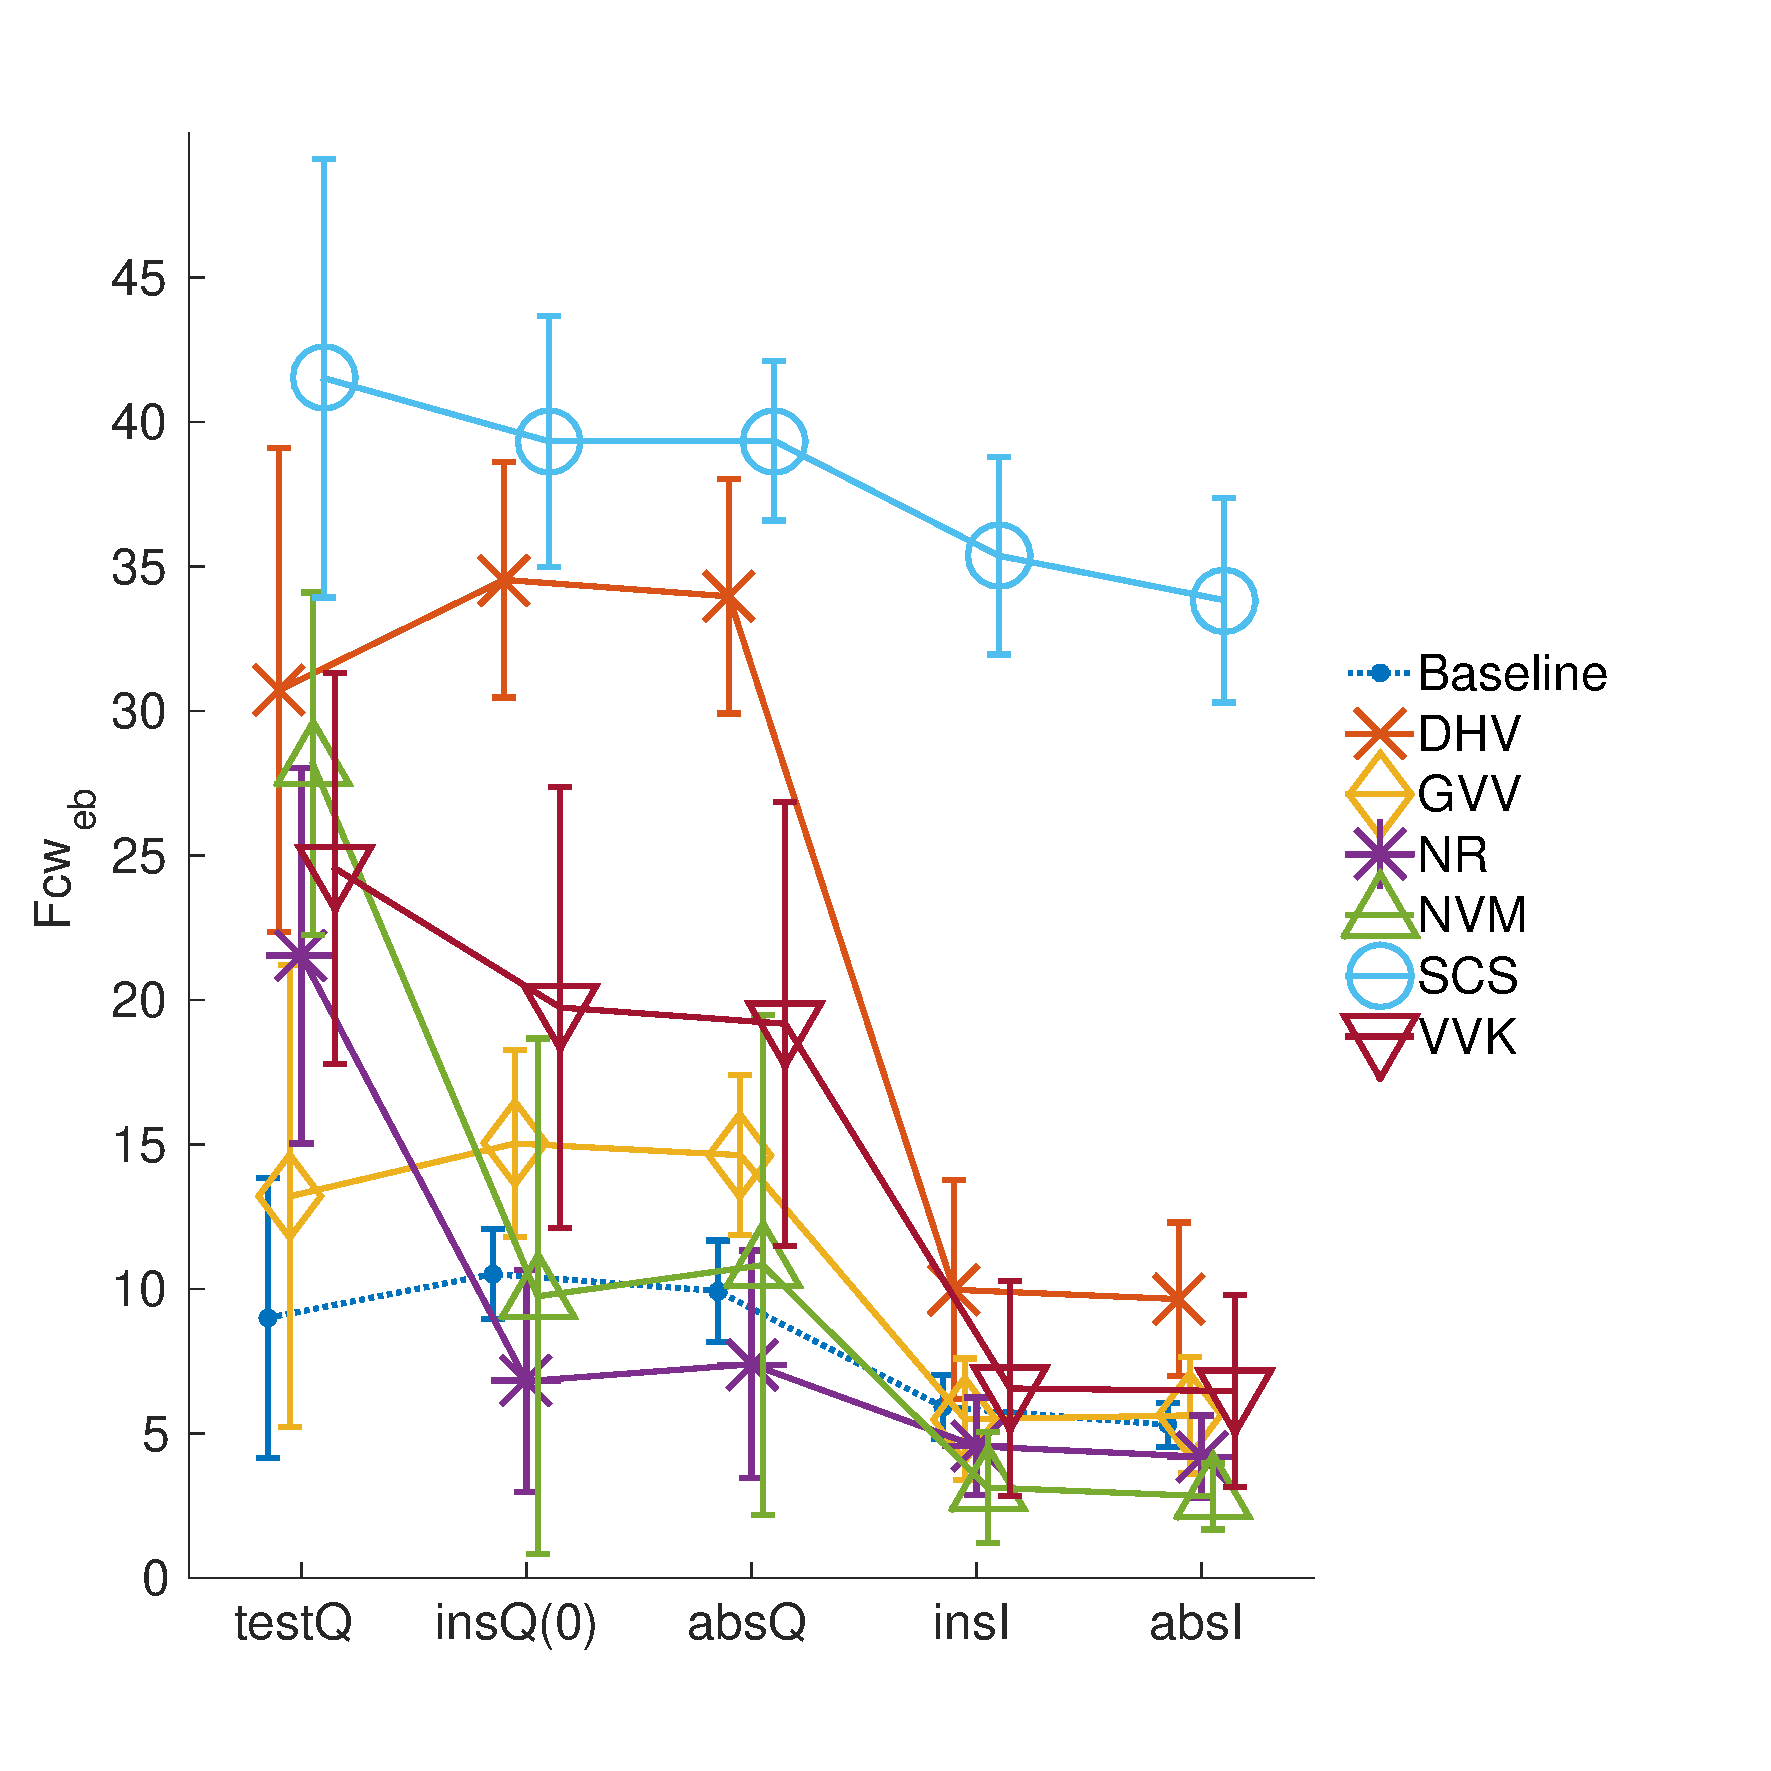
\includegraphics[width=1\columnwidth]{gfx/ch_7/dcase2013_1}
\caption{Performances des systèmes évaluées dans le cadre du challenge DCASE 2013 sur les corpus QMUL et IRCCYN en considérant $Fcw_{eb}$.}
\label{fig:irccyn}
\end{figure}

\subsubsection{Corpus QMUL}

\begin{table}[t] 
\begin{center}  
\begin{tabular}{lccc}  
Système  & testQ & insQ-EBR(0) & absQ \\ 
\hline 
Baseline & 9.0$\pm$4.8      & 10.5$\pm$3.0$^*$     & 9.9$\pm$3.5 \\ 
CPS      & 0.7$\pm$0.8      & 0.8$\pm$1.3          & 0.8$\pm$1.4$^*$ \\ 
DHV      & 30.7$\pm$8.4     & 34.5$\pm$7.5$^*$     & 34.0$\pm$7.9 \\ 
GVV      & 13.2$\pm$8.0     & 15.0$\pm$6.4$^*$     & 14.6$\pm$6.2 \\ 
NR       & 21.5$\pm$6.5$^*$ & \textbf{6.8$\pm$5.7} & \textbf{7.4$\pm$5.8} \\ 
NVM      & 28.2$\pm$5.9$^*$ & \textbf{9.7$\pm$9.6} & \textbf{10.8$\pm$9.9} \\ 
SCS      & 41.5$\pm$7.6$^*$ & 39.3$\pm$8.2         & 39.4$\pm$8.2 \\ 
VVK      & 24.6$\pm$6.8$^*$ & 19.7$\pm$8.7         & 19.2$\pm$9.2 \\  
\hline
\end{tabular} 
\end{center} 
\caption[Résultats mesurés par $Fcw_{eb}$ pour chacun des systèmes évalués dans le cadre du challenge DCASE 2013 en considérant les corpus \emph{test-QMUL}, \emph{insQ-EBR(0)} et \emph{abstract-QMUL}.]{Résultats mesurés par $Fcw_{eb}$ pour chacun des systèmes évalués dans le cadre du challenge DCASE 2013 en considérant les corpus \emph{test-QMUL}, \emph{insQ-EBR(0)} et \emph{abstract-QMUL}. Les résultats en gras présentent des différences significatives par ligne (procédure de Tukey-Kramer) avec le résultat obtenu pour \emph{test-QMUL}. Le meilleur résultat de la ligne est indiqué par ($^*$).} 
\label{tab:qmul} 
\end{table} 

Avec la permission des auteurs des différents systèmes proposés (\cf~Tableau~\ref{tab:systemsDcase2013}), ces derniers sont testés sur les corpus de scènes simulées, en utilisant les mêmes serveurs de calculs que ceux utilisés pour la tache 2 (AED) du challenge DCASE 2013. Les systèmes ont par ailleurs été re-testés sur le corpus \emph{test-QMUL} (corpus de \emph{test} du challenge AED DCASE 2013), afin de vérifier la réplicabilité des résultats précédemment publiés \citep{Stowell15}.

Le Tableau~\ref{tab:qmul} affiche les $Fcw_{eb}$ en pourcentages pour les corpus \emph{test-QMUL}, \emph{insQ-EBR(0)} et \emph{abstract-QMUL}. Le système CPS, tel que soumis au challenge DCASE 2013, présente un problème d'implémentation l'empêchant de fonctionner correctement. Ce problème est à l'origine des faibles résultats obtenus pour \emph{test-QMUL}, résultats qui se retrouvent sur \emph{insQ-EBR(0)} et \emph{abstract-QMUL}. Pour ces raisons nous ne considérons pas plus avant ce système.

\gl{L'ANOVA montre un effet significatif du corpus  ($F[2,30]=6$, $p<0.01$), des systèmes  ($F[6,180]=173$, $p_{gg}<0.01$) et de l'interaction  ($F[12,180]=10$, $p_{gg}<0.01$). Il semble ainsi au premier abord que le changement de corpus a bien provoqué une modification des performances, et ce bien que les sons utilisés pour simuler les corpus \emph{abstract-QMUL} et \emph{insQ-EBR(0)} soient similaires à ceux que l'on trouve dans \emph{test-QMUL}.}

\gl{Cependant, l'analyse \emph{post hoc} au niveau des corpus révèle que la \emph{Baseline}, DHV, GVV, SCS et VVK ne présentent pas de différences significatives entre les performances observées pour \emph{test-QMUL} d'une part, et celles relevées pour \emph{abstract-QMUL} et \emph{insQ-EBR(0)} d'autre part. Seules les résultats de NVM et NR décroissent significativement entre \emph{test-QMUL} et les deux corpus simulés.}

Ainsi, exception faite de NR et NVM, les classements des systèmes établis par rapport à leur performances sont égaux pour les 3 corpus. Ces résultats permettent de conclure deux points quant aux performances de DHV, GVV, SCS et VVK:

\begin{itemize}
\item comparaison entre \emph{test-QMUL} et \emph{insQ-EBR(0)}: les performances comparables montrent que les algorithmes sont robustes au changement d'événements. À noter que les samples proviennent tous des enregistrements de QMUL, \ie~ont été enregistrés dans les mêmes conditions;
\item comparaison entre \emph{test-QMUL} et \emph{abstract-QMUL}: les performances comparables montrent que les algorithmes sont robustes à un changement de positions temporelles des samples, si les paramètres structuraux des scènes ($EBRs$ et espacements inter-\emph{onsets}) sont conservés.
\end{itemize}
  
\begin{table}[t]
\begin{center} 
\begin{tabular}{lllllll}  
  Système &   testQ         &  insQ-EBR(0)      &   absQ          \\
 \hline
 Baseline & 3.14            &  8.63             &  7.40    \\
          & (tiroir)        &  (tiroir)         & (tiroir) \\
      CPS & 2.66            &  9.04             &  7.84   \\
          & (porte-frapper) & (porte-claquer)   & (porte-claquer) \\
      DHV & 8.44            &  6.88             &  8.01  \\
          & (tiroir)        &  (tiroir)         &  (clavier)  \\
      GVV & 3.08            &  3.78             &  3.55   \\
          & (page)          &  (page)           & (page) \\
      NR  & 4.33            & \textbf{25.35}    & \textbf{20.68}  \\
          & (clavier)       & (porte-claquer)   & (porte-claquer)  \\
      NVM & 1.26            & \textbf{22.48}    & \textbf{19.22}    \\
          & (rire)          & (toux)            & (toux) \\
      SCS & 1.18            &  2.70             &  1.72   \\
          & (alerte)        &  (tiroir)         & (porte-claquer)  \\
      VVK & 1.81            &  8.73             &  8.20   \\ 
          & (alerte)        &  (porte-claquer)  & (porte-claquer) \\
       \hline
\end{tabular}
\end{center} 
\caption[Nombre maximum de faux positifs pour chaque système évalué et pour chaque corpus]{Nombre maximum de faux positifs pour chaque système évalué et pour chaque corpus. Les résultats sont moyennés suivant les enregistrements. Les classes de sons correspondantes sont indiquées entre parenthèses.}
\label{tab:fp}
\end{table}

Nous examinons maintenant les raisons pouvant expliquer les chutent de performances des systèmes NVM et NR dans le cas des scènes simulées. En effet, la chute peut être due soit à l'incapacité des algorithmes à généraliser sur d'autres corpus, soit à un artefact produit par les processus de simulation.

Pour chacun des algorithmes, la première étape consiste à extraire des descripteurs sur l'ensemble des trames du signal, la seconde consiste à classifier ces trames.

Considérons dans un premier temps les descripteurs extraits. Les valeurs minimales et maximales ne varient pas entre \emph{test-QMUL} et les corpus de scènes simulées. Les distributions des valeurs des descripteurs entre les deux types de corpus présentent certes une différence, mais cette dernière se révèle faible et non-significative. 

Une inspection des matrices de confusion inter-classes révèle que c'est, pour les deux systèmes, l'étape de classification qui serait responsable de la dégradation des performances. Le tableau~\ref{tab:fp} affiche, pour tous les systèmes, le plus grand nombre de faux positifs moyennés sur l'ensemble des scènes pour les trois corpus, ainsi que la classe correspondante. Pour NVM et NR, une classe en particulier (NVM: toux, NR: porte-claquer) semble être détectée de manière abusive, augmentant drastiquement le nombre de faux positifs, et diminuant \emph{de facto} les résultats.

Nous concluons que, pour ces deux systèmes, la diminution des performances n'est probablement pas un artefact dû au processus de simulation, mais plutôt a un phénomène de sur-apprentissage de l'étape de classification. Considérant que ces systèmes sont les seuls à faire usage d'une approche de classification discriminative (NR: SVMs; NVM: RFs), nous conjecturons que le cadre d'entraînement proposé par le challenge DCASE, et notamment le faible nombre de samples disponibles pour l'apprentissage (20 par classe), n'est pas adapté pour ces deux algorithmes.

\subsubsection{Corpus instance-QMUL en considérant différents niveaux de bruit}

\begin{figure}[t]
\begin{center}
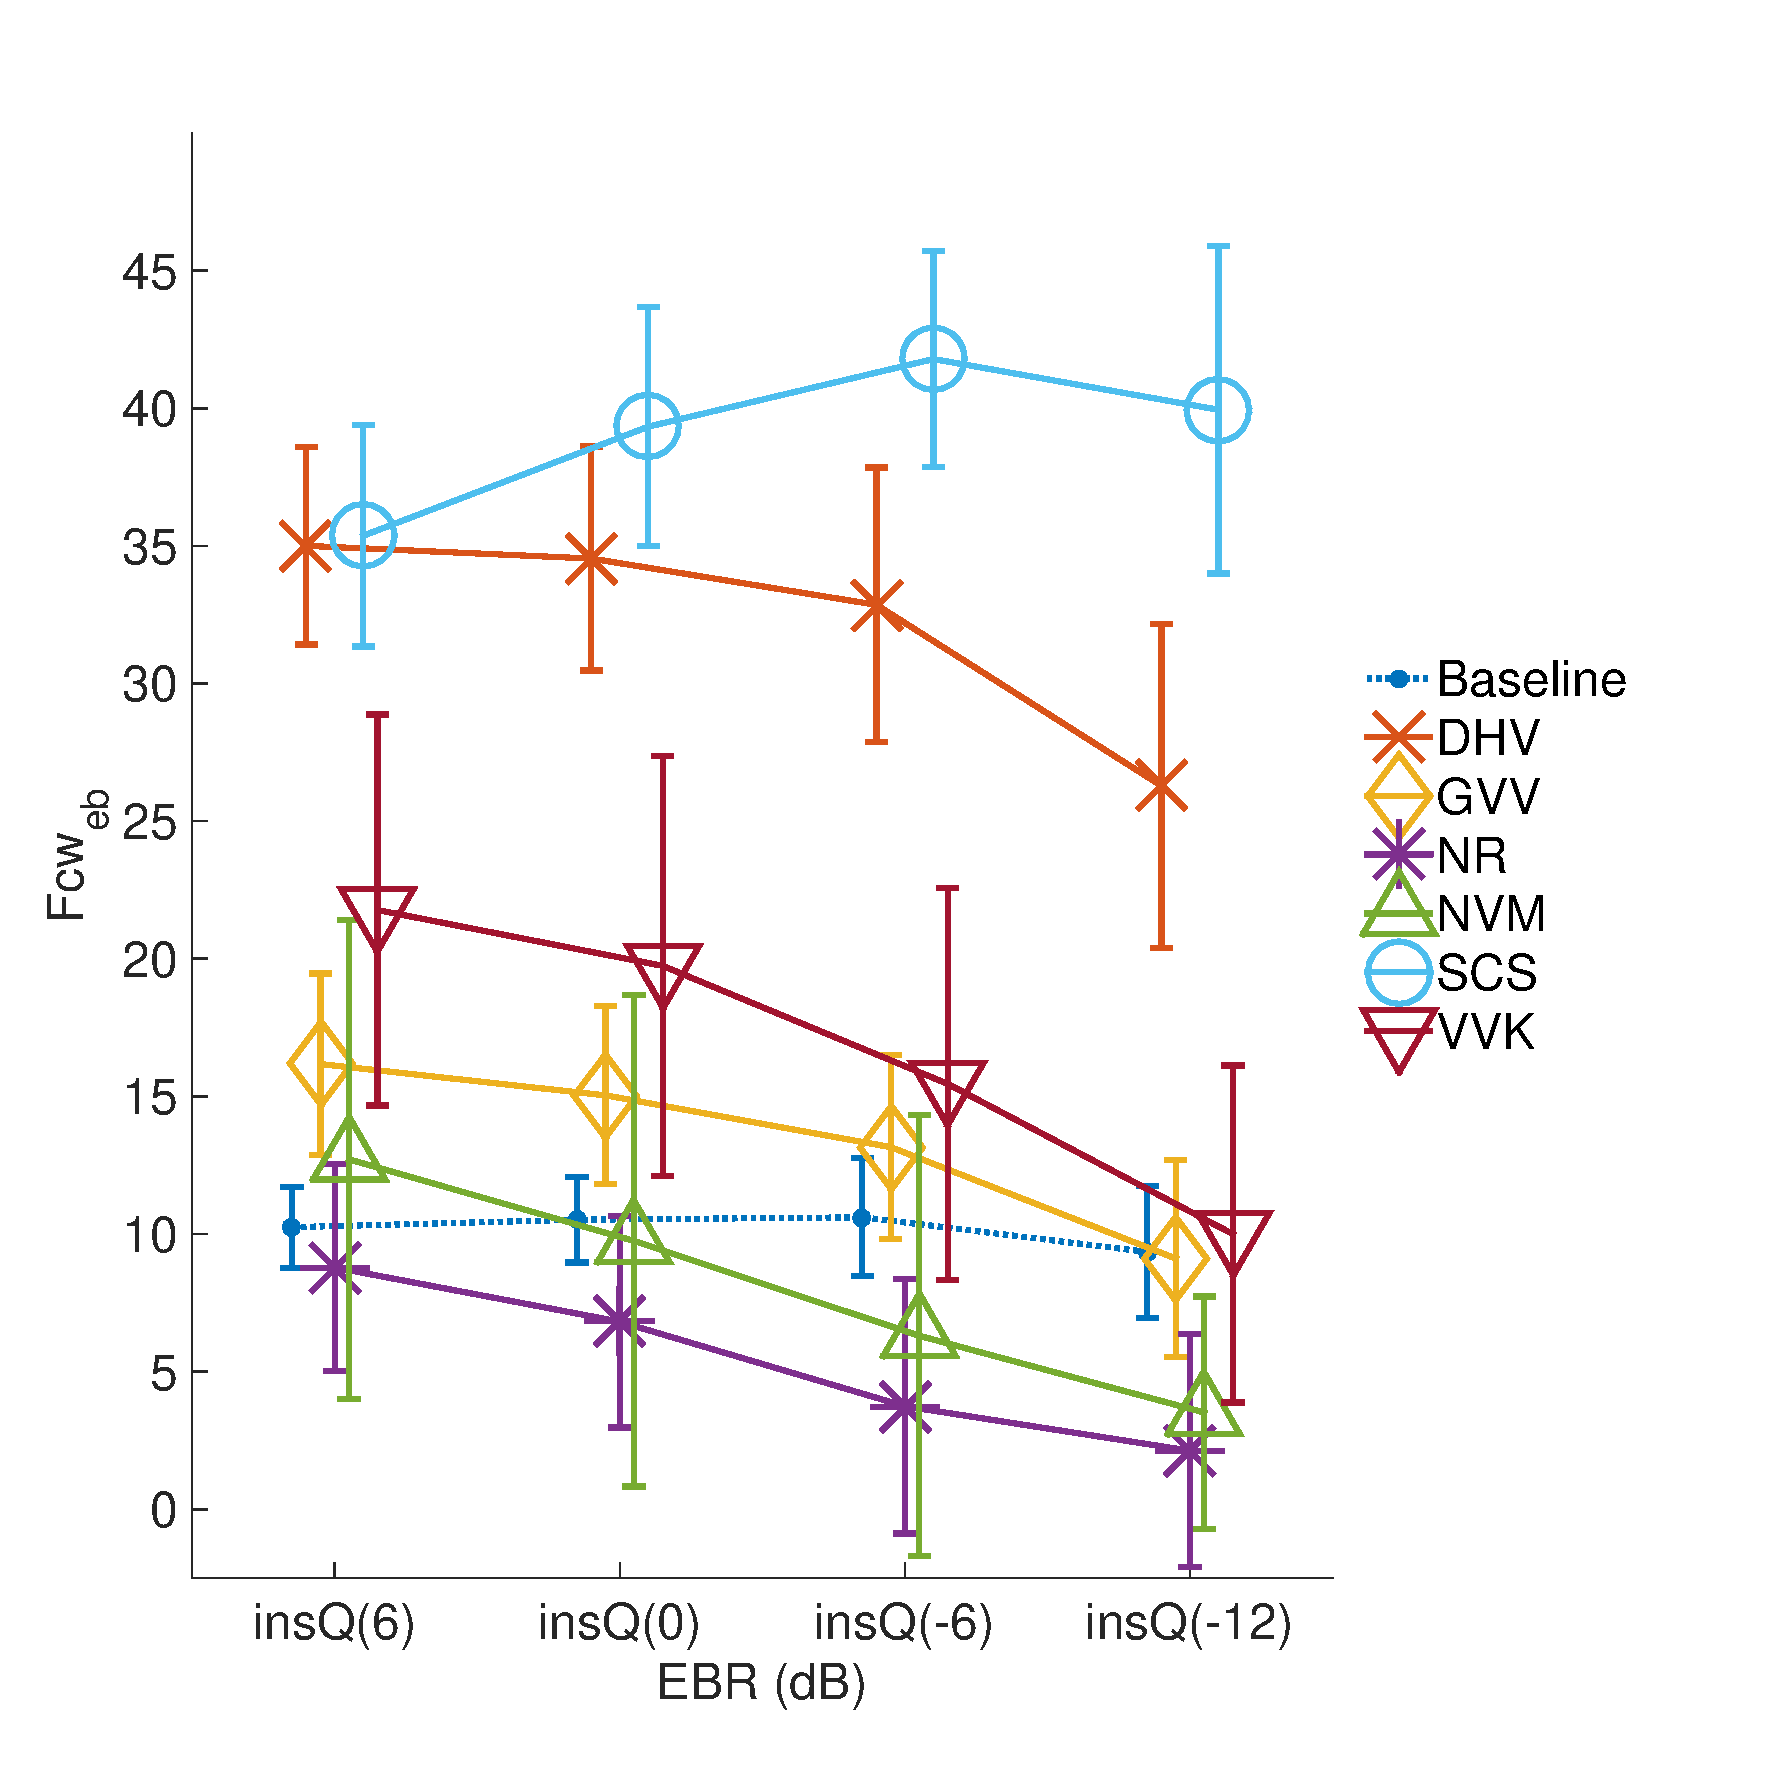
\includegraphics[width=1\columnwidth]{gfx/ch_7/dcase2013_2}
\caption{Performances des systèmes évaluées dans le cadre du challenge DCASE 2013 sur les corpus \emph{instance-QMUL} simulés avec différents $EBR$ ($6$, $0$, $-6$ et $-12dB$).}
\label{fig:ebr} 
\end{center}
\end{figure}

Nous considérons maintenant l'influence de l'$EBR$ sur les performances des algorithmes. Les résultats obtenus pour les corpus \emph{insQ-EBR(-12)}, \emph{insQ-EBR(-6)}, \emph{insQ-EBR(0)} et \emph{insQ-EBR(6)} (\cf~Section~\ref{sec:ch7_datasetEtEbr}) sont présentés sur la figure~\ref{fig:ebr}. 

\gl{L'ANOVA reporte un effet significatif de l'$EBR$ ($F[3,30]=63$, $p_{gg}<0.01$), des systèmes ($F[6,60]=128$, $p_{gg}<0.01$) et de l'interaction ($F[18,180]=16$, $p_{gg}<0.01$).}

\gl{Concernant l'analyse \emph{post hoc} entre $EBR$, tous les systèmes affichent une dégradation de performances significative lorsque l'on passe d'un $EBR$ de $0dB$ à un $EBR$ de $-12dB$, ainsi qu'une amélioration significative lorsque l'on passe d'un $EBR$ de $0dB$ à un $EBR$ de $+6dB$ (excepté DHV qui ne présente pas l'amélioration significative). Ainsi, et sans surprise, plus l'$EBR$ est faible, et plus les performances diminuent. Par ailleurs, plus l'$EBR$ est faible, et plus les écarts entre les algorithmes se réduisent. Le seul système qui ne suit pas cette tendance est SCS, qui maintient des performances stables pour les différents $EBRs$, et améliore même significativement ces dernières pour des $EBRs$ allant de $6$ à -6$dB$. Ces résultats montrent l'efficacité de l'étape de dé-bruitage substantielle dont bénéficie SCS, pré-traitement qui est au cœur de son algorithme \citep{SCS}.} \\

\gl{TODO: expliquer pourquoi la baseline ne varie pas ?} \\

\gl{L'influence de l'$EBR$ est cependant cohérente, le classement en termes de performances entre les algorithmes étant maintenu pour les différents corpus.} 

\gl{Concernant l'analyse \emph{post hoc} entre systèmes, seuls DHV et SCS présentent des performances significativement supérieures à celles de la \emph{baseline}, et ce quelque soit l'$EBR$ considéré. VVK et GVV arrivent à surpasser la \emph{baseline} uniquement pour des $EBR$ de $0dB$ et $6dB$, \ie~des niveaux de bruit faibles. Concernant NR et NVM, ces systèmes n'améliorent jamais significativement les résultats de la \emph{baseline}, et affichent même des performances significativement inférieures à celle-ci pour des $EBR$ de $-12$ (NR et NVM) et de $-6dB$ (NR), montrant ainsi leur faible capacité de généralisation pour des niveaux de bruit élevés.}

\gl{Ces résultats nous amènent à conclure que à part SCS, aucun des systèmes considérés n'est robuste aux différents niveaux de bruit.}
\subsubsection{Corpus IRCCYN}

\begin{table}
\begin{center} 
\begin{tabular}{lccc}
Système  & testQ            & insI                   & absI \\ 
\hline 
Baseline & 9.0$\pm$4.8$^*$  &  \textbf{5.9$\pm$2.9}  &  \textbf{5.6$\pm$2.9} \\ 
DHV      & 30.7$\pm$8.4$^*$ &  \textbf{10.0$\pm$5.8} &  \textbf{9.5$\pm$5.6} \\ 
GVV      & 13.2$\pm$8.0$^*$ &  \textbf{5.6$\pm$3.7}  &  \textbf{5.5$\pm$3.6} \\
NR       & 21.5$\pm$6.5$^*$ &  \textbf{4.6$\pm$3.4}  &  \textbf{5.4$\pm$4.5} \\ 
NVM      & 28.2$\pm$5.9$^*$ &  \textbf{3.1$\pm$3.1}  &  \textbf{3.2$\pm$3.0} \\ 
SCS      & 41.5$\pm$7.6$^*$ &  \textbf{35.4$\pm$7.2} & \textbf{34.0$\pm$6.7} \\ 
VVK      & 24.6$\pm$6.8$^*$ &  \textbf{6.6$\pm$5.7}  &  \textbf{7.3$\pm$6.3} \\ 
\hline
\end{tabular} 
\end{center}  
\caption[Résultats mesurés par $Fcw_{eb}$ pour chacun des systèmes évalués dans le cadre du challenge DCASE 2013 en considérant les corpus \emph{test-QMUL}, \emph{instance-IRCCYN} et \emph{abstract-IRCCYN}.]{Résultats mesurés par $Fcw_{eb}$ pour chacun des systèmes évalués dans le cadre du challenge DCASE 2013 en considérant les corpus \emph{test-QMUL}, \emph{instance-IRCCYN} et \emph{abstract-IRCCYN}. Les résultats en gras présentent des différences significatives par ligne (procédure de Tukey-Kramer) avec le résultat obtenu pour \emph{test-QMUL}. Le meilleur résultat de la ligne est indiqué par ($^*$).}
\label{tab:irccyn} 
\end{table} 

\gl{Les résultats sont affichés sur le tableau~\ref{tab:irccyn} et la figure~\ref{fig:irccyn}. L'ANOVA montre un effet significatif du corpus  ($F[2,30]=89$, $p<0.01$), des systèmes  ($F[6,180]=249$, $p_{gg}<0.01$) et de l'interaction  ($F[12,180]=17$, $p_{gg}<0.01$).}

\gl{Concernant l'analyse \emph{post hoc} relatif aux corpus, alors que la plupart des systèmes ont obtenu des performances comparables entre \emph{test-QMUL} et les corpus \emph{abstract-} et \emph{instance-QMUL}, tous algorithmes voient leurs résultats diminuer de manière significative pour les corpus  \emph{abstract-} et \emph{instance-IRCCYN}}.

\gl{De plus, l'analyse \emph{post hoc} des systèmes révèle que, à l'exception du système SCS, tous les systèmes ont des résultats équivalents ou significativement inférieurs (NVM) à ceux de la \emph{baseline} pour les deux corpus \emph{IRCCYN}. En particulier le système DHV, qui pourtant montre de bons résultats pour les corpus \emph{QMUL}}.

L'ensemble de ces résultats nous permet de conclure que, pour les systèmes DHV, GVV, NR, NVM et VVK, le gain de performance par rapport à la baseline observé sur le corpus \emph{test-QMUL} n'est dû qu'à une sur-adaptation des systèmes aux données d'entraînement (corpus d'entraînement et de développement du challenge DCASE 2013). 

Comme on peut clairement le voir sur la figure~\ref{fig:irccyn}, seul le système SCS (gagnant du challenge AED DCASE 2013), arrive à maintenir des performances stables entre tous les corpus considérés. Cette capacité de généralisation est par ailleurs cohérente, le système parvenant en effet à généraliser quelque soit la condition expérimentale que l'on fait varier, nommément: 

\begin{itemize}
\item les samples sélectionnés (en considérant deux banques de sons isolés différentes);
\item les positions temporelles des samples;
\item les $EBRs$.
\end{itemize}

\subsection{Discussion}

Pour résumer les résultats présentés précédemment, l'utilisation des scènes simulées à partir du modèle de scènes sonores proposé nous a permis de:

\begin{enumerate}
\item reproduire le classement des systèmes dans les mêmes conditions d'enregistrement pour 5 d'entre eux. Les deux systèmes posant problème (NR et NVM) présentent des performances dégradées. Nous montrons que cette dégradation est probablement due à un sur apprentissage de leurs  classifieurs discriminants respectifs;
\item évaluer les capacités de généralisation des systèmes dans de nouvelles conditions d'enregistrement. A cet égard, le système SCS est le seul à généraliser correctement;
\item évaluer la robustesse des systèmes devant traiter des niveaux de bruits de fond différents. Une nouvelle fois, le système SCS est le seul a présenter des performances stables pour les différents $EBR$ considérés, et ce, probablement en raison d'une étape efficace de pré-traitement du bruit .
\end{enumerate}

L'ensemble de ces résultats montre l'utilité des processus de simulation proposés (\cf~Sections~\ref{sec:ch7_simuProcessAbstract} et~\ref{sec:ch7_simuProcessInstance}), ces derniers permettant bien de répliquer ou d'aller plus loin dans l'analyse des performances des algorithmes.

À la lumière de ces résultats, nous pensons que, tenir compte de données soigneusement simulées est utile afin d'acquérir plus de connaissances sur les propriétés et les comportements des systèmes en cours d'évaluation, connaissance pouvant ainsi aider les chercheurs dans leurs choix algorithmiques. 

Les facteurs influant sur les performances tels que le niveau de bruit, le niveau de polyphonie, la diversité intra-classe (différence acoustique entre la formation et les données d'essais) peuvent ainsi être évalués de façon indépendante, sans avoir la charge 

\begin{enumerate}
\item d'enregistrer des scènes présentant les propriétés désirées;
\item d'annoter manuellement les données.
\end{enumerate}

Même si l'usage exclusif de données simulées, pour valider une approche algorithmique, est insuffisant, nous pensons que la seule utilisation de données réelles ne permet pas non plus d'acquérir des connaissances sur l'impact de certains problèmes de conception et de paramétrisation rencontrés dans la mise en œuvre d'un système d'ingénierie. Les données réelles sont, la plupart du temps, des ressources rares, la conception minutieuse d'un grand ensemble de données d'évaluation étant une tâche très exigeante. En outre, l'annotation a posteriori de la présence des événements doit être effectuée par par des individus dont le consensus n'est pas garanti. L'utilisation de données de simulation est un entre deux, qui, combiné à une validation sur données réelles, permet d'obtenir une meilleure compréhension des systèmes en cours d'évaluation. 

%%%%%%%%%%%%%%%%%%%%%%%%%%%%%%%%%%%%%%%%%%%%%%%%%%%%%%%%%%%%%%%%%%%%%%%%%%%%%%%%%%%%%%%%%%%%%%%
%%%%%%%%%%%%%%%%%%%%%%%%%%%%%%%%%%%%   DCASE 2016   %%%%%%%%%%%%%%%%%%%%%%%%%%%%%%%%%%%%%%%%%%%
%%%%%%%%%%%%%%%%%%%%%%%%%%%%%%%%%%%%%%%%%%%%%%%%%%%%%%%%%%%%%%%%%%%%%%%%%%%%%%%%%%%%%%%%%%%%%%%

\section{Application au challenge DCASE  2016}

\subsection{Objectifs}

Nous présentons dans cette section les résultats de la tâche 2 du challenge DCASE 2016\footnote{\cf~\url{http://www.cs.tut.fi/sgn/arg/dcase2016/}}, la seconde édition du challenge DCASE 2013. La tâche 2 est nommée ``\,détection d'événements sonores dans des environnements simulées\,''\footnote{\cf~\url{http://www.cs.tut.fi/sgn/arg/dcase2016/task-sound-event-detection-in-synthetic-audio}}. Cette tâche 2 a été réalisée dans le cadre de notre thèse. 

L'objectif est ici d'évaluer les performances d'algorithmes en AED sur des corpus de scènes simulées, scènes dont nous contrôlons:

\begin{itemize}
\item l'intensité des événements sonores;
\item le nombre d'événements sonores par scènes.
\end{itemize}

Par ailleurs nous faisons la distinction entre deux types de scènes, à savoir:

\begin{itemize}
\item les scènes autorisant le recouvrement entre les événements de classes différentes;
\item les scènes n'autorisant pas le recouvrement.
\end{itemize}

\subsection{Génération des corpus}

\subsubsection{Banque de sons isolés}

\begin{table}[t]
\begin{center}
\begin{tabular}{lcc}
\textbf{Index} & \textbf{Nom}  & \textbf{Description}  \\ 
\hline
1   & porte-frapper & Frapper à la porte \\
2   & porte-claquer & Claquer la porte \\
3   & parole        & Personne  prononçant une phrase \\
4   & rire          & Personne riant  \\    
5   & gorge         & Personne se raclant la gorge  \\
6   & toux          & Personne toussant \\
7   & tiroir        & Ouverture/fermeture d'un tiroir \\
8   & clavier       & Bruit des touches d'un clavier \\
9   & clefs         & Poser un jeu de clefs sur une table \\    
10  & téléphone     & Sonnerie de téléphone \\
11  & page          & Tourner une page \\     
\hline      
\end{tabular}
\end{center}
\caption{Classes d'événements sonores utilisées dans le cadre du challenge DCASE 2016}
\label{tab:eventDCASE2016}
\end{table}

La banque de données de sons isolés \emph{IRCCYN} (\cf~Section~\ref{sec:ch7_eventDataset}) a été utilisée pour simuler les scènes. 11 classes d'événements sont considérées dans le cadre de cette tâche. Les classes sont décrites dans le tableau~\ref{tab:eventDCASE2016}. Comparé au challenge DCASE 2013, 5 classes ont été supprimées:

\begin{itemize}
\item alerte: la classe a été supprimée en raison de sa définition trop ``\,vague\,''. En effet la diversité des sons pouvant appartenir à la classe alerte électronique est importante;

\item bouton, souris, stylo: ces classes ont été supprimées après analyse des résultats du challenge DCASE 2013. En effet, lors de ce dernier, ces classes:

\begin{enumerate}
\item ont souvent été confondues entre elles;
\item ont souvent été très mal détectées. 
\end{enumerate}

\item imprimante: cette classe a été supprimée en raison de son aspect singulier par rapport aux autres classes. En effet, la classe imprimante est composée de sons significativement plus longs que ceux des autres classes. Un tel déséquilibre rend difficile un contrôle équitable du nombre d'événements par classe, pour chaque scène, particulièrement dans le cas où le recouvrement entre les événements est interdit.

\end{itemize}

\subsubsection{Simulation des scènes sonores}
\label{sec:ch7_simulationDcase2016}

Deux paramètres sont considérés pour contrôler la simulation des scènes sonores:

\begin{itemize}
\item $EBR$: le rapport moyen entre les niveaux des événements et du \emph{background} (\cf~Section~\ref{sec:ch7_simuProcessInstance});
\item $nombre d'événement$ ($nec$): le nombre d'événements présents pour chaque classe;
\end{itemize}

Contrairement à ce qui s'était fait pour les scènes simulées du Challenge DCASE 2013, nous ne considérons plus l'espacement moyen entre les \emph{onsets} des événements pour contrôler la densité d'événements présents, mais directement le nombre d'événements ($nec$). Ainsi, nous garantissons que chaque classe soit représentée par le même nombre d'événements, indépendamment de leurs durées.

Par ailleurs, les $EBRs$ des événements sont constants, \ie~fixer un $EBR$ de -6$dB$ pour une scène revient à fixer un $EBR$ de -6$dB$ pour chaque événement de cette scène.

Enfin, deux types de scènes sont considérés. Les scènes polyphoniques, scènes où les événements de différentes classes peuvent se recouvrer, et les scènes non-polyphoniques, scènes où un seul événement peut être actif à un moment donné.

Pour chaque scène, la position des \emph{onsets} des événements est tirée aléatoirement, suivant une distribution uniforme. Dans le cas des scènes non-polyphoniques, une étape de post-traitement assure qu'aucun événement ne se recouvre.

Nous considérons trois niveaux pour les paramètres $EBR$ et $nec$. Pour $nec$. Les valeurs de ces niveaux dépendent de la nature polyphonique de la scène:

\begin{itemize}
\item $EBR$: -6, 0 et +6$dB$;
\item $nec$: 
\begin{itemize}
\item non-polyphonique: 1, 2 et 3;
\item polyphonique: 3, 4 et 5.
\end{itemize}
\end{itemize}

L'ensemble des valeurs des paramètres nous donne 18 conditions expérimentales (3 $EBR$ $\times$ 3 $nec$ $\times$ 2 polyphonie). À noter cependant que, comme pour les scènes simulées du challenge DCASE 2013, une modification de l'$EBR$ n'affecte que ce denier, \ie~les positions des \emph{onsets} et les samples sélectionnés ne sont pas modifiés.

\subsubsection{Banque d'entraînement}

La banque d’entraînement comprend 220 sons isolés, 20 pour chacune des classes considérées.

\subsubsection{Corpus de développement}

Les scènes du corpus de développement sont simulées à partir des sons isolés d'événements de la banque d’entraînement, auxquels nous ajoutons 1 son de \emph{Background}

Nous simulons une scène pour chacune des 18 conditions expérimentales définies par les paramètres de contrôle (\cf~Section~\ref{sec:ch7_simulationDcase2016}), nous donnant ainsi un corpus formé de 18 scènes sonores simulées.

Concernant la sélection des samples d'événements, ces derniers sont différents pour chaque valeur de $nec$ et de polyphonie. Autrement dit, un changement de $nec$, ou de nature polyphonique, modifie l'ensemble des samples de la scène. 

Un même sample de \emph{background} est utilisé pour simuler l'ensemble des scènes de la banque de développement.

\subsubsection{Corpus d'évaluation}

Les scènes du corpus d'évaluation sont simulées à partir d'une banque de sons isolés composée de 440 sons d'événements, 40 pour chacune des classes considérées, et 3 sons de \emph{background}.

Pour chacune des 18 conditions expérimentales définies par les paramètres de contrôle (\cf~Section~\ref{sec:ch7_simulationDcase2016}), la simulation est répliquée trois fois, nous donnant ainsi un corpus de 54 scènes sonores simulées (18 $\times$ 3). Pour chaque réplication, la position des \emph{onsets} est retirée. Les graines des générateurs aléatoires sont différentes de celles employées pour simuler le corpus de développement.

Concernant les samples d'événements sélectionnés, ces derniers sont différents pour chaque valeur de $nec$, de polyphonie et chaque $replication$. 
 
Concernant les samples de \emph{background}, ces derniers sont différents pour chaque $replication$. 

Les scènes ont toutes une durée de 2 minutes. La durée total du corpus est ainsi de 108 minutes.

\subsection{Métrique}

Parmi les 4 métriques utilisées dans le cadre du challenge DCASE 2016 (\cf~Section~\ref{sec:ch6_metriqueAED}), nous en choisissons 1 dans le cadre de cette analyse:

\begin{itemize}
\item $Fcw_{eb}$: la F-mesure, calculée en prenant en compte les \emph{onsets} des événements, et en normalisant les résultats par classe.
\end{itemize}

L'identification des \emph{onsets} des événements est effectuée avec une fenêtre de tolérance de 200 ms.

\subsection{Données et analyses}

Les métriques sont calculées séparément sur chacune des scènes du corpus d'évaluation, et moyennées en fonction des conditions expérimentales considérées. Ce que faisant, nous nous éloignons de l'évaluation officielle réalisée pour le challenge 2016, où le calcul des métriques est effectué sur l'ensemble des scènes, \ie~en considérant que toutes les scènes n'en forment qu'une.

L'analyse s'effectue en trois temps:

\begin{itemize}
\item dans un premier temps, nous considérons les résultats sans tenir compte des différentes conditions expérimentales ($nec$ et $EBR$). Il s'agit ici d'apprécier les performances globales des algorithmes. Les différences entre les systèmes sont appréciées à l'aide d'une ANOVA à mesures répétées (\cf~Annexe~\ref{app:anova}) à un facteur (les différents systèmes);
\item dans un second temps, nous considérons les résultats entre les scènes polyphoniques et les scènes non-polyphoniques, sans toutefois prendre en compte $nec$ et $EBR$. Les différences entre les systèmes sont appréciées à l'aide d'une ANOVA à mesures répétées (\cf~Annexe~\ref{app:anova}) comportant 1 facteur intra-sujet (\emph{within subject}: les différents systèmes) et 1 facteur inter-sujet (\emph{between subject}: la polyphonie); 
\item dans un troisième temps, nous évaluons l'impact des différentes conditions expérimentales ($nec$, $EBR$) sur les performances des algorithmes, en considérant séparément les scènes polyphoniques, et les scènes non-polyphoniques. Pour $nec$, les différences entre les systèmes sont appréciées à l'aide d'une ANOVA à mesures répétées (\cf~Annexe~\ref{app:anova}) comportant 1 facteur intra-sujet (\emph{within subject}: les différents systèmes) et 1 facteur inter-sujet (\emph{between subject}: $nec$). Pour $EBR$ cependant, les différences sont appréciées à l'aide d'une ANOVA à mesures répétées à deux facteurs intra-sujets (les différents systèmes et $EBR$). En effet, les samples et les positions des \emph{onsets} n'étant pas modifiés lors d'un changement d'$EBR$, il existe clairement une relation de dépendance entre les différents niveaux d'$EBR$. Nous n'évaluons jamais les deux conditions expérimentales $nec$ et $EBR$ en même temps, les observations disponibles (au nombre de trois) n'étant pas jugées suffisantes.
\end{itemize}

Pour les ANOVA à mesures répétées, la sphéricité est évaluée à l'aide d'un test de Mauchly. Si l'hypothèse de sphéricité est violée, la valeur $p$ est calculée à l'aide d'une correction de Greenhouse-Geisser (\cf~Annexe~\ref{app:anova}). Dans ce cas, nous notons $p_{gg}$ la valeur $p$ ainsi corrigée. L'analyse \emph{post hoc} est conduite en suivant la procédure de Tukey-Kramer. Un seuil de significativité de $\alpha=0.05$ est choisi.

\subsection{Systèmes de détection}

\begin{table}[t]
\begin{center}
\scriptsize
\begin{tabular}{lcccc}
\textbf{Système}             & \textbf{Descripteur}         & \textbf{Classifieur} &   \multicolumn{2}{c}{Gestion du bruit} \\ 
                             &                              &                      & réduction & apprentissage   \\ 
\hline
\emph{Komatsu}               &     VQT                      & NMF-MLD              &           & x \\ 
\citep{Komatsu2016}          &                              &                      &           &   \\ 
\hline
\emph{Choi}                  &     mel                      & DNN                  & x         & x \\ 
\citep{Choi2016}             &                              &                      &           & \\ 
\hline
\emph{Hayashi 1}             &     mel                      & BLSTM-PP             &           & x \\ 
\citep{Hayashi2016}          &                              &                      &           & \\ 
\hline
\emph{Hayashi 2}             &     mel                      & BLSTM-HMM            &           & x \\ 
\citep{Hayashi2016}          &                              &                      &           & \\ 
\hline
\emph{Phan}                  &     GTCC                     & RF                   &           & x\\ 
\citep{Phan2016}             &                              &                      &           & \\ 
\hline
\emph{Giannoulis}            &     mel                      & CNMF                 &           & x\\ 
\citep{Giannoulis2016}       &                              &                      &           & \\ 
\hline
\emph{Pikrakis}              &     Bark                     & Template             & x         & \\ 
\citep{Pikrakis2016}         &                              & matching             &           & \\ 
\hline
\emph{Vu}                    &     CQT                      & RNN                  &           & \\ 
\citep{Vu2016}               &                              &                      &           & \\ 
\hline
\emph{Gutierrez}             &     MFCC                     & Knn                  &           & x \\ 
\citep{GutierrezArriola2016} &                              &                      &           & \\ 
\hline
\emph{Kong}                  &     mel                      & DNN                  &           &  \\ 
\citep{Kong2016}             &                              &                      &           & \\ 
\hline  
\emph{Baseline}              &     VQT                      & NMF                  &           & \\ 
\citep{Benetos2016}          &                              &                      &           & \\ 
\hline 
\end{tabular}
\end{center}
\caption{Description synthétique des systèmes soumis dans le cadre de la tâche 2 du challenge DCASE 2016}
\label{tab:systemsDcase2016}
\end{table}

Cette section décrit les systèmes soumis à la tâche 2 du challenge DCASE 2013. 10 algorithmes sont proposés, auxquels nous rajoutons la \emph{baseline}. Une description synthétique de ces systèmes est donnée au tableau~\ref{tab:systemsDcase2016}. 

Concernant les descripteurs, on peut regrouper les algorithmes en 5 groupes:

\begin{itemize}
\item \emph{mel/bark}: une représentation temps-fréquence, où l'axe fréquentiel à été projeté sur une échelle particulière, soit de Bark (\emph{Pikrakis}; \cf~section~\ref{sec:ch6_Bark}) soit de Mel (\emph{Choi}, \emph{Hayashi 1}, \emph{Hayashi 2}, \emph{Giannoulis} et \emph{Kong}; \cf~Section~\ref{sec:ch6_Mel});
\item \emph{VQT/CQT}: une représentation temps-fréquence calculée en \gl{TODO}(\cf~Section~\ref{sec:ch6_VQT_CQT});
\item \emph{MFCC}: : une représentation basée sur des coefficients cepstraux calculés sur échelle de Mel (MFCCs: \emph{Mel-Frequency Cepstral Coefficients}; \cf~Section~\ref{sec:ch6_mfcc}).
\item \emph{GTCC}: une représentation basée sur des coefficients cepstraux calculés sur échelle de Gammatone (GTCCs: \emph{Gammatone cepstral coefficients}; \cf~Section~\ref{sec:ch6_Gammatone}).
\end{itemize}

Concernant les classifieurs utilisés, on distingue 6 groupes:

\begin{itemize}
\item \emph{Réseaux de neurones}: \emph{Kong} et \emph{Choi}  \gl{TODO};
\item \emph{Factorisation de matrices non négatives}: \emph{Komatsu}, \emph{Giannoulis} et \emph{baseline}   \gl{TODO};
\item \emph{BLSTM}: \emph{Hayashi 1} et \emph{Hayashi 2} \gl{TODO};
\item \emph{Arbre de décision}: \emph{Phan} \gl{TODO};
\item \emph{Plus proches voisins}: \emph{Gutierrez} \gl{TODO};
\item \emph{Template matching}: \emph{Pikrakis} \gl{TODO}.
\end{itemize}

\subsection{Résultats}

\subsubsection{Analyse globaux}
\label{sec:ch7_analyseGlobaleDcase2016}

\begin{figure}[t]
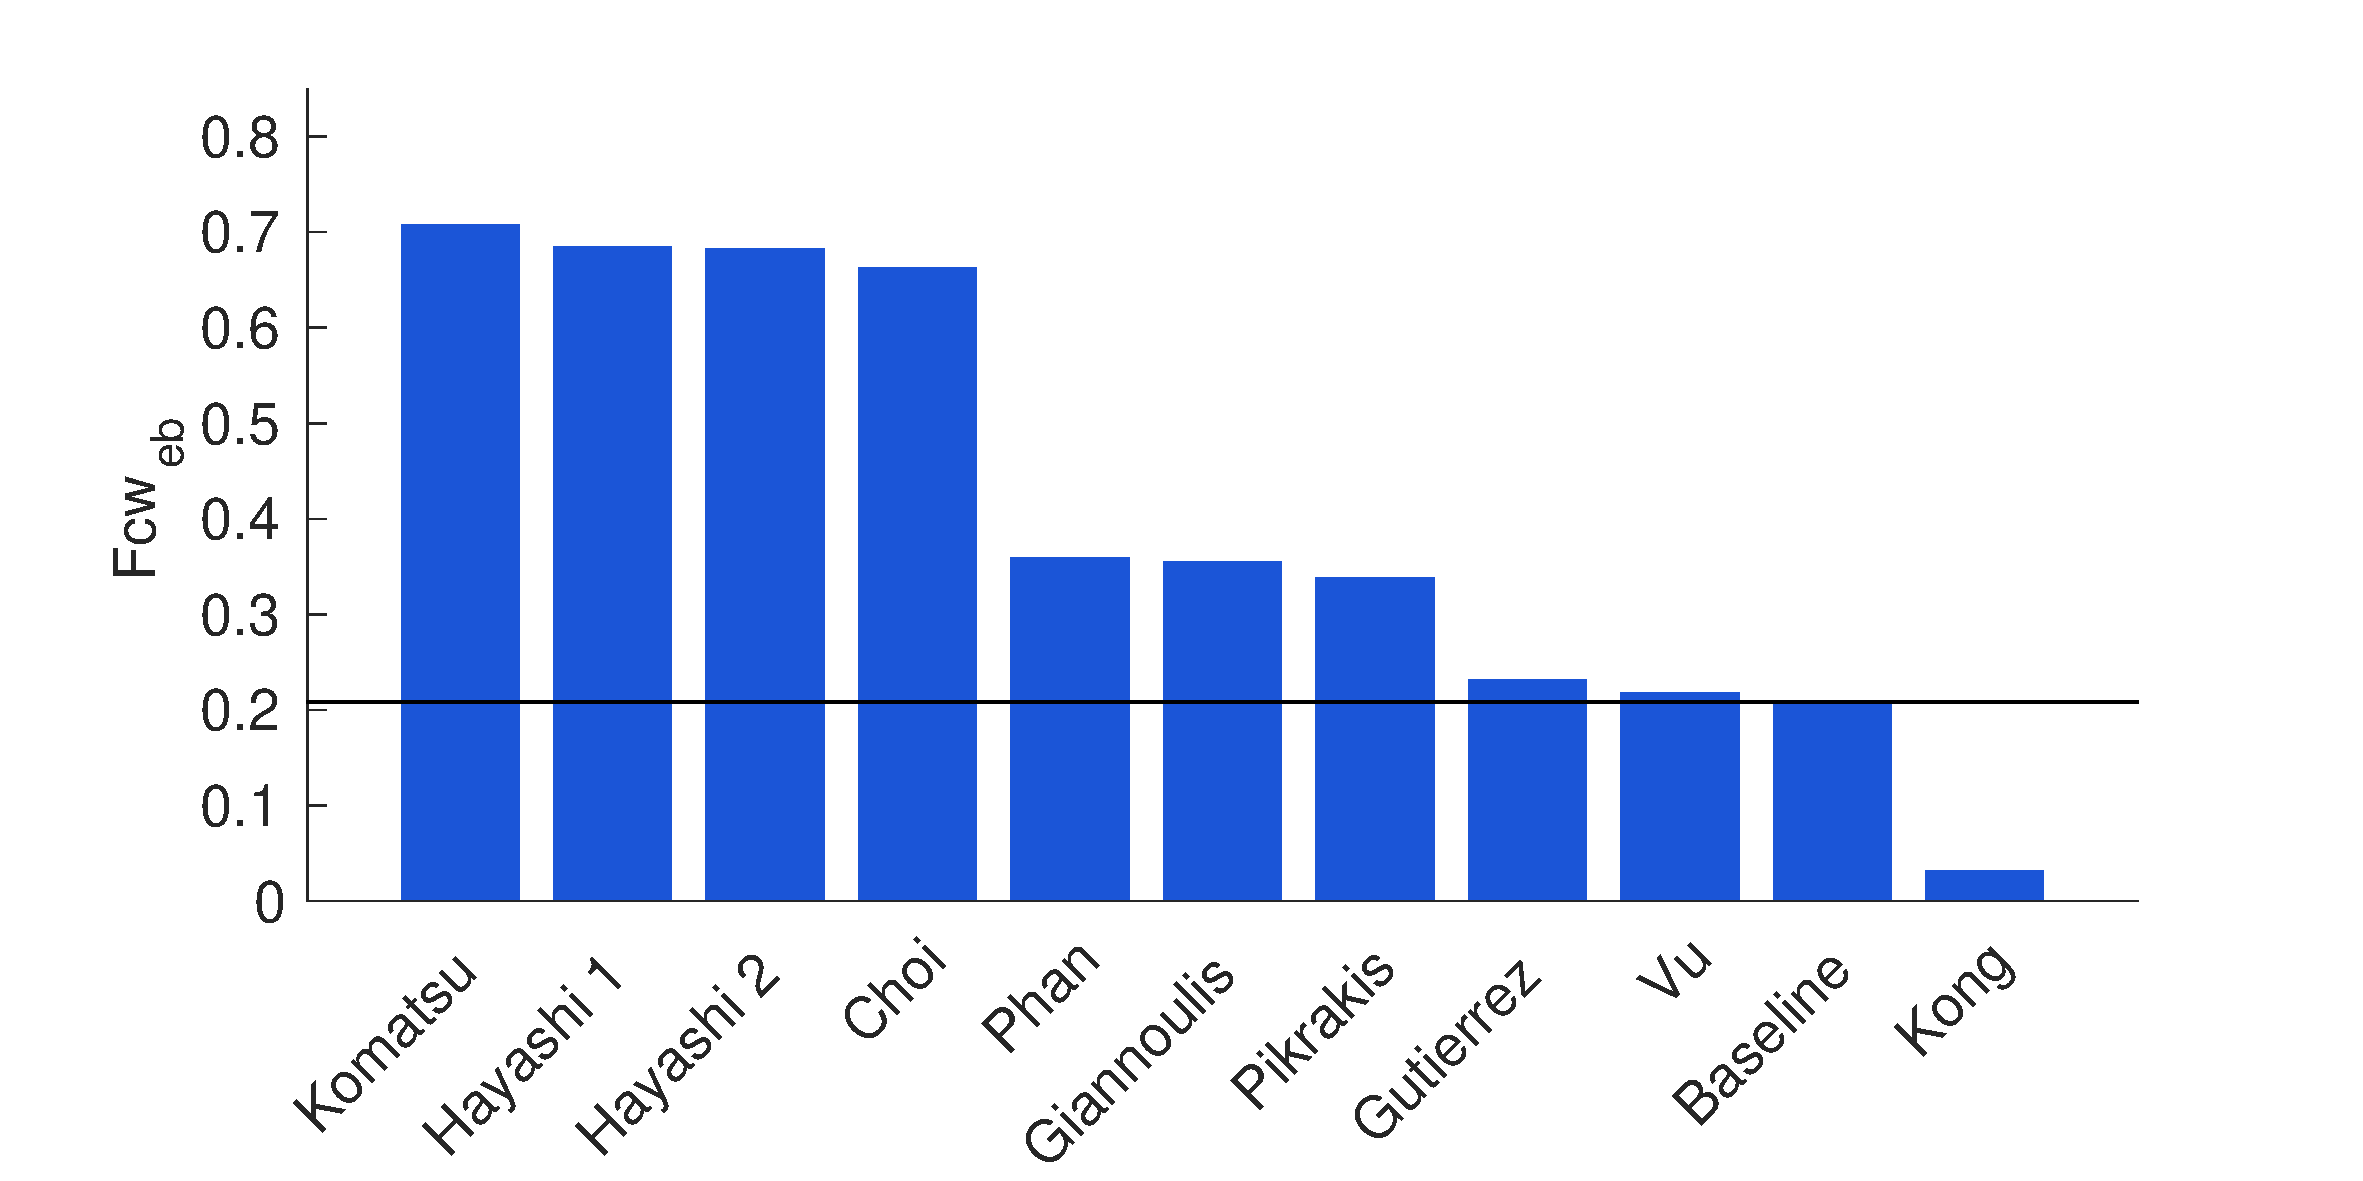
\includegraphics[width=1\textwidth]{gfx/ch_7/results_overall_eb_class_wise_average_F_6}
\caption{Performances globales des algorithmes évalués dans le cadre de la tâche 2 du challenge DCASE 2016, en considérant la métrique $Fcw_{eb}$.}
\label{fig:overall_eb_class_wise_F}
\end{figure}

Les résultats globaux sont affichés sur la figure~\ref{fig:overall_eb_class_wise_F}. L'ANOVA pratiquée sur $Fcw_{eb}$ révèle un effet positif du type de système ($F[10,530]=466$, $p_{gg}<0.01$). L'analyse \emph{post hoc} nous permet d'isoler 4 groupes de systèmes, les systèmes d'un même groupe ne présentant pas de différences significatives dans leurs résultats:

\begin{enumerate}
\item \emph{Komatsu}, \emph{Hayashi 1}, \emph{Hayashi 2} et \emph{choi}: les performances moyennes allant de 67\% (\emph{choi}) à 71\% (\emph{Komatsu});
\item \emph{Phan}, \emph{Giannoulis} et \emph{Pikrakis}: les performances moyennes allant de 34\% (\emph{Pikrakis}) à 36\% (\emph{Phan});
\item \emph{Baseline}, \emph{Vu} et \emph{Gutierrez}: les performances allant de 21\% (\emph{Baseline}) à 23\% (\emph{Gutierrez});
\item \emph{Kong}: la performance moyenne étant de 22\%;
\end{enumerate}

Ainsi sur les 10 systèmes soumis, 7 parviennent à surpasser les résultats présentés par la \emph{Baseline}, les systèmes du groupe 2 affichant une amélioration d'environ 15\%, ceux du groupe 1 améliorant les résultats de près de 45\%.

Il est difficile de dégager l'influence d'un classifieur particulier, les systèmes du groupe 1 faisant usage de DNN, de NMF et de BLSTM. Pour les descripteurs cependant, 3 systèmes sur 4 du groupe 1 utilisent des bandes de Mel. Notons également l'importance, pour le système, de considérer le bruit (\emph{background}), soit en le modélisant, soit en réduisant ce dernier sur les données à évaluer. En effet, les trois systèmes n'ayant pas tenu compte de l'influence du bruit présentent les trois performances les plus faibles.

Le système affichant les résultats les moins bons est \emph{Kong}. Ce dernier est le seul a présenter des résultats systématiquement en deçà de la \emph{baseline}. Une explication possible de ces faibles performances: la phase d'apprentissage du DNN utilisé \citep{Kong2016}. En effet, l’entraînement d'un tel classifieur nécessite un grand nombre de données afin d'être robuste, \ie~capable de généraliser. Or la banque d'entraînement proposée dans le cadre de cette tâche est loin d'être suffisante. 

L'autre système faisant usage d'un DNN (\emph{Choi}) applique, lui, une étape d'augmentation de données, visant à augmenter artificiellement le nombre d'items sur lesquels entraîner l'algorithme \citep{Choi2016}. Ce qui manque dans l'apprentissage de \emph{Kong}. Nous ne considérons pas plus avant les résultats de ce système dans la suite de l'analyse.

\subsubsection{Influence de la polyphonie}

\begin{figure}[t]
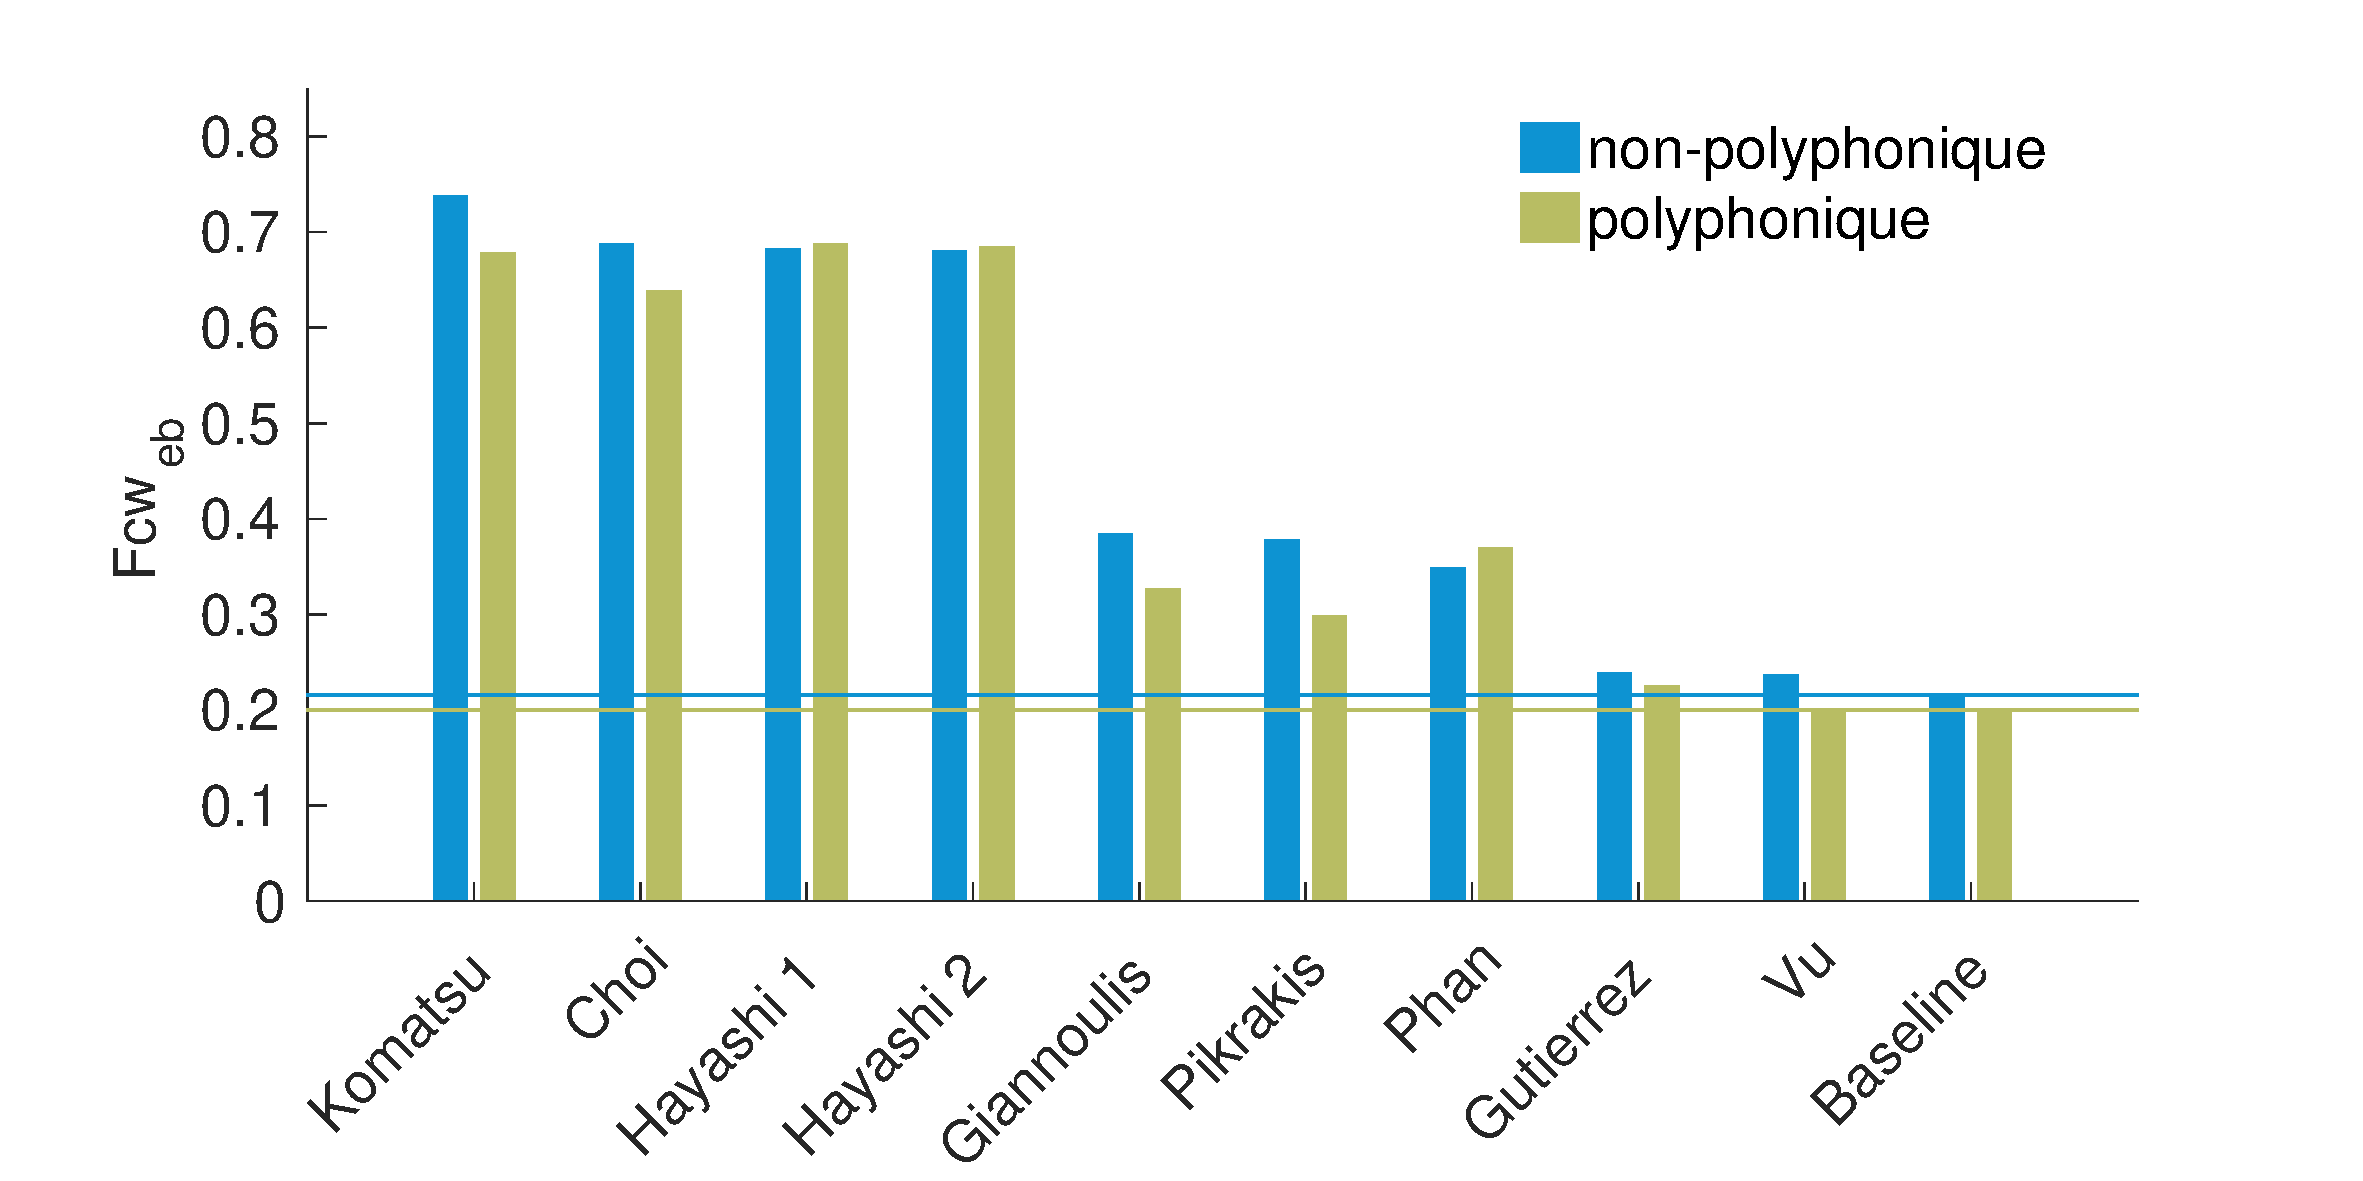
\includegraphics[width=1\textwidth]{gfx/ch_7/results_overall_poly_eb_class_wise_average_F_7}
\caption{Influence de la polyphonie sur les performances des algorithmes évalués dans le cadre de la tâche 2 du challenge DCASE 2016, en considérant la métrique $Fcw_{eb}$.}
\label{fig:overall_poly_eb_class_wise_F}
\end{figure}

Les résultats par types de scènes (polyphoniques et non-polyphoniques) sont affichés sur la figure~\ref{fig:overall_poly_eb_class_wise_F}. L'ANOVA pratiquée sur $Fcw_{eb}$ révèle un effet positif du type de système ($F[9,468]=358$, $p_{gg}<0.01$), mais pas de la polyphonie ($F[1,52]=3.5$, $p=0.07$). Un effet d'interaction est néanmoins constaté ($F[10,520]=2.5$, $p_{gg}<0.05$).

Ainsi, la qualité polyphonique des scènes n'a pas affecté les performances des algorithmes, ces derniers étant capables de gérer de manière équivalente les deux cas de figures. L'analyse \emph{post hoc} sur le facteur polyphonique nous indique que sur les 10 systèmes considérés, 4 affichent des performances différentes, suivant le caractère polyphonique des scènes, nommément  \emph{choi}, \emph{Giannoulis}, \emph{Komatsu} et \emph{Pikrakis}. Pour ces 4 systèmes, le passage au polyphonique dégrade les performances, constat qui était déjà suggéré par l'effet significatif de l'interaction dans l'ANOVA.

L'analyse \emph{post hoc} sur le facteur système nous permet d'isoler les trois mêmes groupes d'algorithmes (le groupe de \emph{Kong} ayant été écarté) que ceux relevés en considérant les résultats globaux (\cf~Section~\ref{sec:ch7_analyseGlobaleDcase2016}), s'agissant des scènes polyphoniques, ou s'agissant des scènes non polyphoniques. Une seule différence est néanmoins notée au niveau des scènes polyphoniques: les systèmes \emph{Gutierrez} et \emph{Pikrakis} ne présentant plus de différences significatives dans ce cas.

\subsubsection{Influence du niveau de bruit}

\begin{figure}[t]
        \myfloatalign
        \subfloat[]
        {\includegraphics[width=1\linewidth]{gfx/ch_7/results_ebr_poly0_eb_class_wise_average_F_5}\label{fig:results_ebr_poly0_eb_class_wise_F}}\par
        \subfloat[]
        {\includegraphics[width=1\linewidth]{gfx/ch_7/results_ebr_poly1_eb_class_wise_average_F_9}\label{fig:results_ebr_poly1_eb_class_wise_F}}\par
       \caption[Influence du niveau de bruit ($EBR$) sur les performances des algortihmes évalués dans le cadre de la tâche 2 du challenge DCASE 2016, en considérant la métrique $Fcw_{eb}$]{Influence du niveau de bruit ($EBR$) sur les performances des algortihmes évalués dans le cadre de la tâche 2 du challenge DCASE 2016, en considérant la métrique $Fcw_{eb}$; (a) scènes non-polyphoniques, (b) scènes polyphoniques.}\label{fig:dcase2016_poly1_eb_fc}
\end{figure}

Considérant les scènes non-polyphoniques, les résultats sont affichés sur la Figure~\ref{fig:results_ebr_poly0_eb_class_wise_F}. l'ANOVA révèle un effet significatif du type de système ($F[9,72]=80$, $p_{gg}<0.01$), et de l'$EBR$ ($F[2,16]=164$, $p_{gg}<0.01$), ainsi que de l'interaction ($F[18,144]=6.5$, $p_{gg}<0.01$). Ainsi plus l'$EBR$ est élevé, plus les performances augmentent, et ce, globalement, pour tous les systèmes.

Concernant l'analyse \emph{post hoc}, nous observons si les systèmes présentent des différences significatives avec la baseline. Pour un $EBR$ de $-6dB$, 4 groupes émergent:

\begin{enumerate}
\item \emph{Komatsu}: performances supérieures à celles de la \emph{Baseline};
\emph{choi}, \emph{Hayashi 1} et \emph{Hayashi 2}: performances supérieures à celles de la \emph{Baseline} mais inférieures à celles du groupe 1;
\item \emph{Gianoulis}: performances supérieures à celles de la \emph{Baseline}, mais inférieures à celles du groupe 1;
\item \emph{Gutierrez}, \emph{Pikrakis}, \emph{Phan} et \emph{Vu}: performances ne présentant pas de différences significatives avec celles de la \emph{Baseline}.
\end{enumerate}

Pour un $EBR$ de $0dB$, trois groupes sont isolés: 

\begin{enumerate}
\item \emph{Komatsu}, \emph{choi}, \emph{Hayashi 1} et \emph{Hayashi 2}: performances supérieures à celles de la \emph{Baseline};
\item \emph{Pikrakis} et \emph{Phan}: performances supérieures à celles de la \emph{Baseline} mais inférieures à celles du groupe 1;
\item \emph{Gutierrez}, \emph{Vu} et \emph{Gianoulis}: performances ne présentant pas de différences significatives avec celles de la \emph{Baseline}.
\end{enumerate}

Enfin, pour un $+6dB$, seulement trois groupes émergent:

\begin{enumerate}
\item \emph{Komatsu}, \emph{choi}, \emph{Hayashi 1} et \emph{Hayashi 2}: performances supérieures à celles de la \emph{Baseline};
\item \emph{Gianoulis}, \emph{Pikrakis} et \emph{Vu}: performances supérieures à celles de la \emph{Baseline} mais inférieures à celles du groupe 1;
\item \emph{Gutierrez} et \emph{Phan}: performances ne présentant pas de différences significatives avec celles de la \emph{Baseline}.
\end{enumerate}

S'agissant des scènes non polyphoniques, il apparaît que le système \emph{Komatsu} permet d'obtenir les meilleures performances, notamment dans les situations de niveau de bruit élevé ($EBR=-6dB$). A noter que seul cet algorithme voit ses performances décroître avec l'$EBR$ (\gl{TODO}), ceci étant dû, sans doute, à l'attention particulière portée par ses auteurs à la modélisation du \emph{Background}.

Les systèmes \emph{choi}, \emph{Hayashi 1} et \emph{Hayashi 2} présentent eux des performances systématiquement supérieures à celles des autres systèmes, et égalent celles de \emph{Komatsu} pour des $EBR$ de $0$ et $+6dB$. Pour ces trois systèmes, l'augmentation du niveau de bruit ($6dB\rightarrow -6dB$) provoque une chute de performances d'environs $10\%$.

Concernant les autres systèmes évalués, \emph{Vu}, \emph{Gianoulis}, \emph{Pikrakis} et \emph{Phan} surpassent la \emph{Baseline} pour certains $EBR$ seulement. Tous ces systèmes semblent souffrir du niveau de bruit, leurs performances diminuant sensiblement avec ce dernier, de $-10$ à $-20\%$ entre un $EBR$ de $6dB$ et un de $-6dB$. Seul \emph{Gutierrez} reste systématiquement au même niveau que la \emph{Baseline}.

S'agissant des scènes polyphoniques, les résultats sont affichés sur la Figure~\ref{fig:results_ebr_poly1_eb_class_wise_F}. l'ANOVA révèle un effet significatif du type de système ($F[9,72]=113$, $p_{gg}<0.01$), et de l'$EBR$ ($F[2,16]=127$, $p_{gg}<0.01$), ainsi que de l'interaction ($F[18,144]=15$, $p_{gg}<0.01$). Encore une fois, plus l'$EBR$ est élevé, plus les performances augmentent, et ce pour tous les systèmes, sauf \emph{Komatsu} .

Pour un $EBR$ de $-6dB$, l'analyse \emph{post hoc} met en évidence 4 groupes de systèmes:

\begin{enumerate}
\item \emph{Komatsu}: performances supérieures à celles de la \emph{Baseline};
\emph{choi}, \emph{Hayashi 1} et \emph{Hayashi 2}: performances supérieures à celles de la \emph{Baseline} mais inférieures à celles du groupe 1;
\item \emph{Gianoulis}: performances supérieures à celles de la \emph{Baseline}, mais inférieures à celles du groupe 1;
\item \emph{Gutierrez}, \emph{Pikrakis}, \emph{Phan} et \emph{Vu}: performances ne présentant pas de différences significatives avec celles de la \emph{Baseline}.
\end{enumerate}

Pour des $EBR$ de $0$ et $-6dB$, trois groupes sont isolés: 

\begin{enumerate}
\item \emph{Komatsu}, \emph{choi}, \emph{Hayashi 1} et \emph{Hayashi 2}: performances supérieures à celles de la \emph{Baseline};
\item \emph{Phan}: performances supérieures à celles de la \emph{Baseline} mais inférieures à celles du groupe 1;
\item \emph{Pikrakis}, \emph{Gutierrez}, \emph{Vu} et \emph{Gianoulis}: performances ne présentant pas de différences significatives avec celles de la \emph{Baseline}.
\end{enumerate}

Les résultats, pour les scènes polyphoniques, sont similaires à ceux obtenus pour les scènes non-polyphoniques. Deux différences sont cependant notées:

\begin{itemize}
\item  \emph{Vu}, \emph{Pikrakis} et \emph{Gutierrez} présentent des résultats équivalents à ceux de la \emph{Baseline} quel que soit l'$EBR$ considéré;
\item  \emph{Phan} semble clairement améliorer ses performances par rapport à celles de la \emph{Baseline} pour des $EBR$ de $0$ et $+6dB$. Ce dernier système souffre ainsi d'une mauvaise prise en compte du bruit, mauvaise prise en compte particulièrement pénalisante dans le cas de scènes polyphoniques ($0dB\rightarrow -6dB$: $41\%\rightarrow 24\%$ )
\end{itemize}

\subsubsection{Influence du nombre d'événements}

\begin{figure}[t]
        \myfloatalign
        \subfloat[]
        {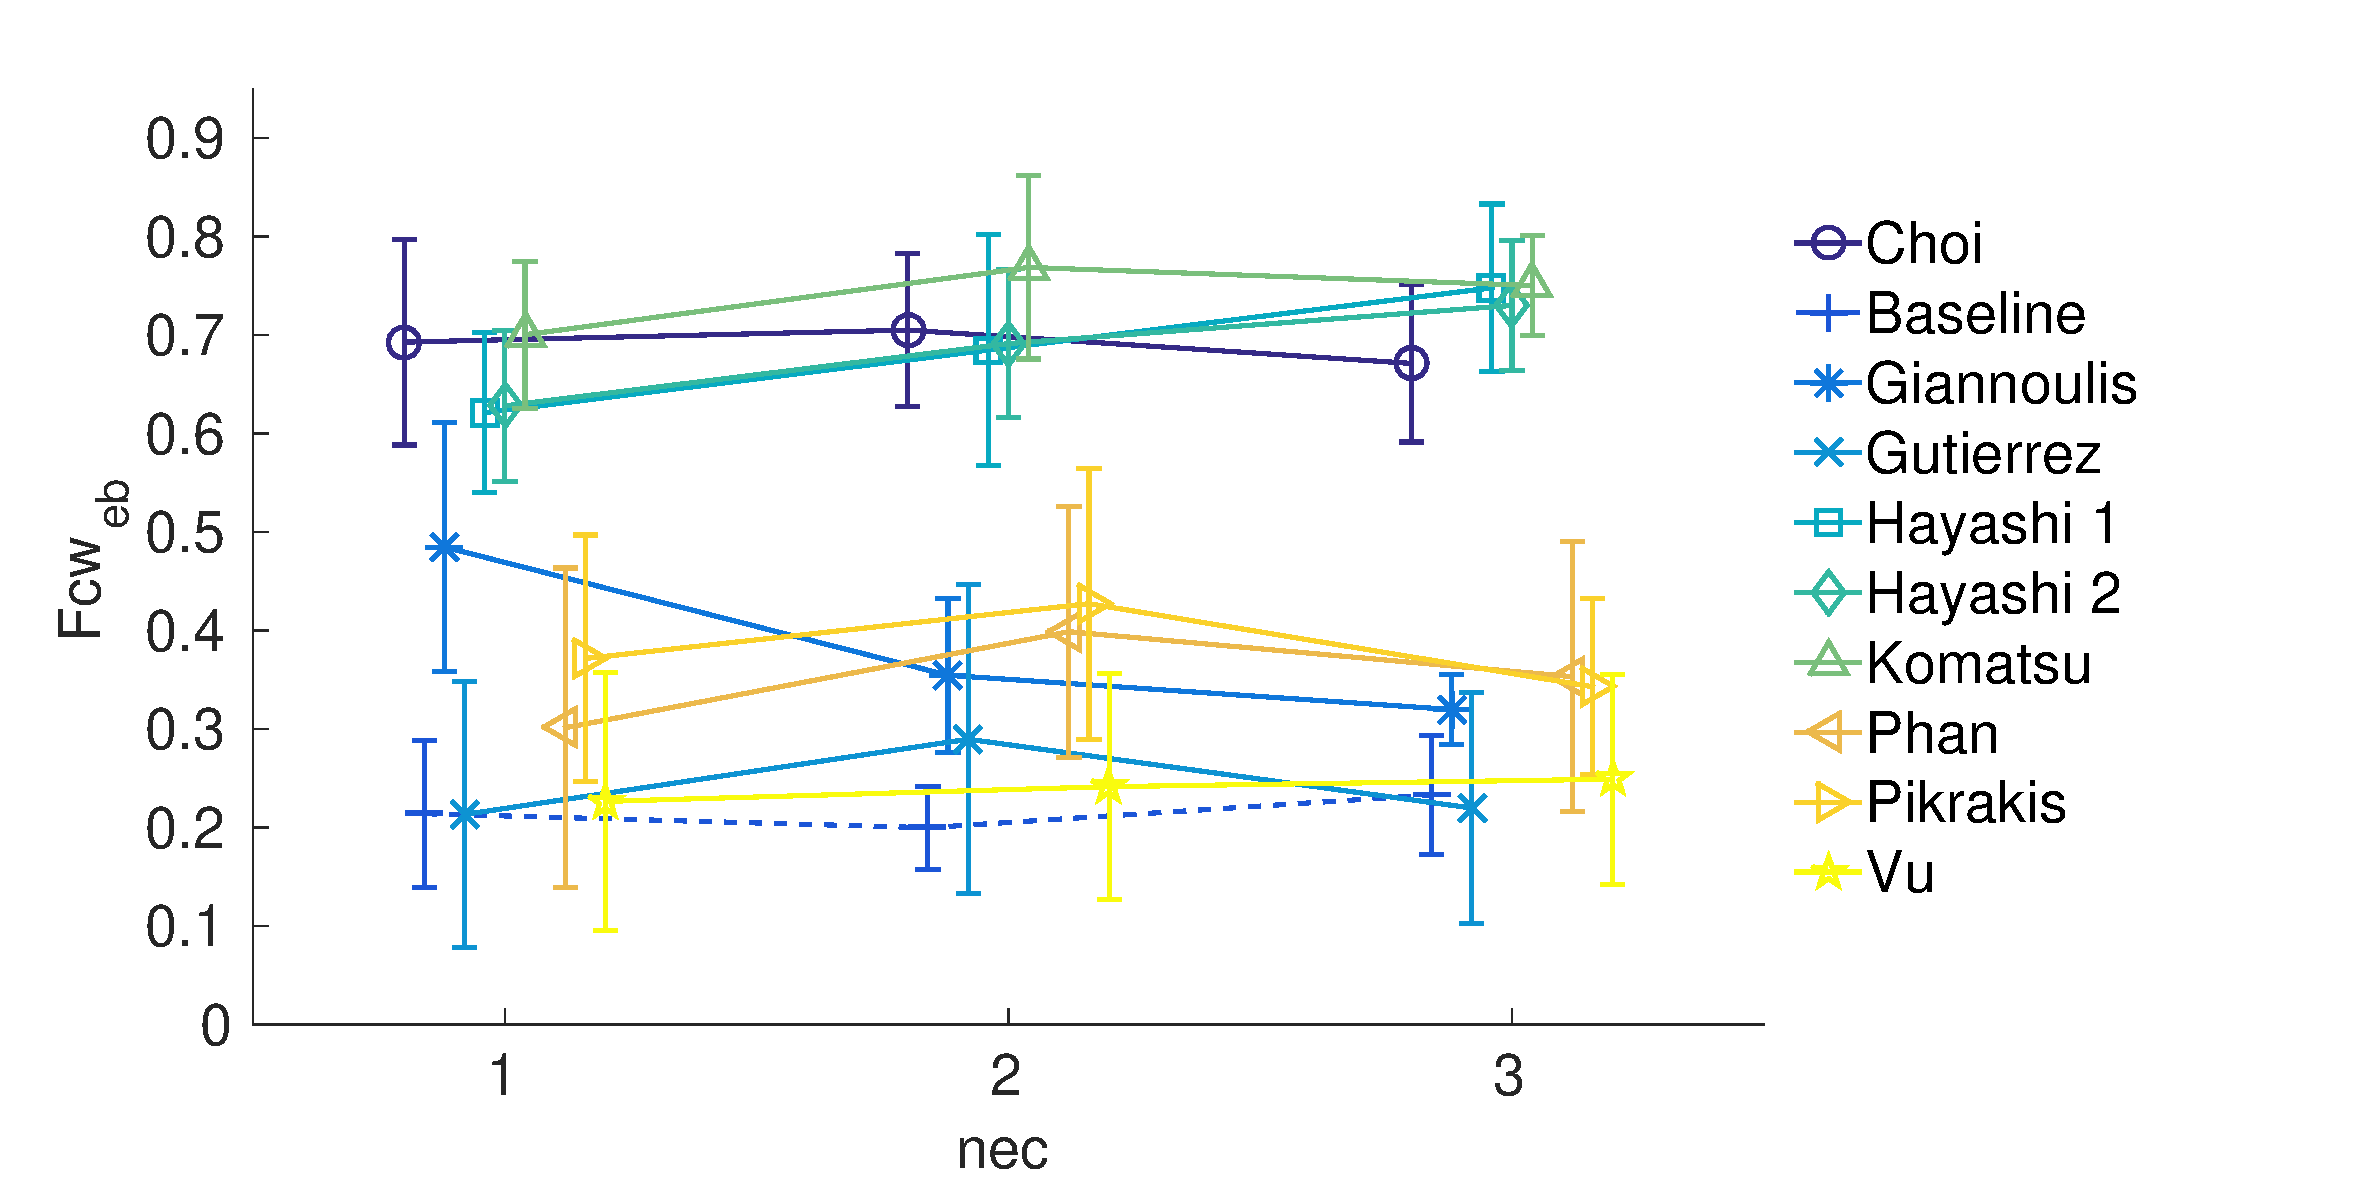
\includegraphics[width=1\linewidth]{gfx/ch_7/results_dens_poly0_eb_class_wise_average_F_5}\label{fig:results_dens_poly0_eb_class_wise_F}}\par
        \subfloat[]
        {\includegraphics[width=1\linewidth]{gfx/ch_7/results_dens_poly1_eb_class_wise_average_F_9}\label{fig:results_dens_poly1_eb_class_wise_F}}\par
       \caption[Influence du nombre d'événements ($nec$) sur les performances des algortihmes évalués dans le cadre de la tâche 2 du challenge DCASE 2016, en considérant la métrique $Fcw_{eb}$]{Influence du nombre d'événements ($nec$) sur les performances des algortihmes évalués dans le cadre de la tâche 2 du challenge DCASE 2016, en considérant la métrique $Fcw_{eb}$; (a) scènes non-polyphoniques, (b) scènes polyphoniques.}\label{fig:results_dens_eb_class_wise_F}
\end{figure}

Considérant les scènes non-polyphoniques, les résultats sont affichés sur la figure~\ref{fig:results_dens_poly0_eb_class_wise_F}. l'ANOVA révèle un effet significatif du type de système ($F[9,216]=264$, $p_{gg}<0.01$), mais pas de $nec$ ($F[2,24]=0.5$, $p=0.6$). Une interaction sensible est néanmoins observée ($F[18,216]=3$, $p_{gg}<0.01$).

Les mêmes résultats sont obtenus pour les scènes polyphoniques (\cf~Figure~\ref{fig:results_dens_poly0_eb_class_wise_F}; système: $F[9,216]=170$, $p_{gg}<0.01$; $nec$: $F[2,24]=0.1$, $p=0.9$; interaction: $F[18,216]=3$, $p_{gg}<0.01$). Ainsi ils nous est difficile de conclure quant à l'influence de $nec$ sur de potentielles différences significatives entre les systèmes.

Malgré tout, nous pouvons isoler certaines tendances. Concernant les scènes non-polyphoniques, l'augmentation du nombre d'événements par classe s'accompagne d'une amélioration systématique des performances pour 2 systèmes ($nec$: $1\rightarrow 3$; \emph{Hayashi 1}: $62\%\rightarrow 75\%$; \emph{Hayashi 2}: $63\%\rightarrow 73\%$) et d'une dégradation pour 1 système ($nec$: $1\rightarrow 3$; \emph{Gianoulis}: $48\%\rightarrow 32\%$). Concernant les scènes polyphoniques, un augmentation est constatée pour 3 systèmes ($nec$: $3\rightarrow 5$; \emph{Hayashi 1}: $67\%\rightarrow 72\%$; \emph{Hayashi 2}: $66\%\rightarrow 73\%$; \emph{Komatsu}: $63\%\rightarrow 70\%$) et une dégradation pour 3 ($nec$: $3\rightarrow 5$; \emph{Gianoulis}: $37\%\rightarrow 27\%$; \emph{Pikrakis}: $36\%\rightarrow 24\%$; \emph{Choi}: $67\%\rightarrow 60\%$).

Alors que l'augmentation du niveau de bruit avait globalement tendance à diminuer les performances des algorithmes, il apparaît que la réaction aux nombres d'événements à détecter varie d'un système à l'autre. Quelle que soit la nature polyphonique des scènes, les systèmes \emph{Hayashi 1} et \emph{Hayashi 2} réagissent systématiquement positivement à l'augmentation du nombre d'événements. Dans le même temps, le système \emph{Gianoulis} voit, lui, ses performances systématiquement décroître.

\subsection{Discussion}

\gl{TODO}
%*****************************************
%*****************************************
%*****************************************
%*****************************************
%*****************************************




